%
%%%%%%%%%%%%%%%%%%%%%%%%%%%%%%%%%%%%%%%%%%%%%%%%%%%%%%%%%%%%%%%%%%%%%%%%%%%%%%%
% Theory
%%%%%%%%%%%%%%%%%%%%%%%%%%%%%%%%%%%%%%%%%%%%%%%%%%%%%%%%%%%%%%%%%%%%%%%%%%%%%%%
%
%\chapter{Quantum Chromodynamics}
\chapter{Theoretical framework}\label{ch:theory}

In this chapter a short overview of the theory of elementary particles and fundamental interactions is presented, with emphasis on the strong interactions and the description of the hadronic final state in hadron collisions.

%------------------------------------------------------------------------
%\section{The theory of the strong interactions}\label{sec:qcdintro}
\section{The Standard Model}\label{sec:qcdintro}
%------------------------------------------------------------------------

The Standard Model (SM) is a quantum field theory that describes the behavior of all experimentally-observed particles under the influence of the electromagnetic, weak and strong forces\footnote{In principle gravitational forces should also be included in the list of fundamental interactions but their impact is  fortunately negligible at the distance and energy scales usually considered in particle physics experiments.}. In this model, all forces of nature are the result of particle exchange. The force mediators interact on the particles of matter, and, in some cases, due to the non-Abelian character of the theory\footnote{The transformations of the symmetry group do not commute in the case of the QCD and weak groups.}, with each other.

Elementary particles are categorized into two classes of particles: \emph{bosons} and \emph{fermions}. Bosons have integer spin and obey the Bose-Einstein statistics, whereas fermions have half-integer spin and follow Fermi-Dirac statistics.  Each elementary particle has a corresponding anti-particle, whose quantum numbers are opposite in sign.

The fundamental building blocks of matter predicted by the SM are fermions with spin $1/2$:

\begin{itemize}\addtolength{\itemsep}{-0.4\baselineskip}
\item
six leptons (and their antiparticles), organized in three families, 

\[ \left( \begin{array}{c} \nu_e \\ e^- \end{array} \right)  \left( \begin{array}{c} \nu_{\mu} \\ \mu^- \end{array} \right)   \left( \begin{array}{c} \nu_{\tau} \\ \tau^- \end{array} \right)     \]


\item
and six quarks (and their antiparticles), organized in three families,

\[ \left( \begin{array}{c} u \\ d \end{array} \right)  \left( \begin{array}{c} c \\ s \end{array} \right)   \left( \begin{array}{c} t \\ b \end{array} \right)     \].
\end{itemize}
These particles are considered point-like, as there is no evidence of any internal structure of leptons or quarks to date. The six types of quarks are also known as the six quark flavors. Collectively, the $u$ (up), $d$ (down), and $s$ (strange) quarks are frequently referred to as the light quarks. The heaviest quark of the Standard Model, the quark $t$ (top), was the last to be found~\cite{PhysRevLett.74.2626,PhysRevLett.74.2422}.  The electric charge\footnote{The electric charge is given in units of the elementary charge, $e$, which is the charge carried by the positron.} $Q$ of quarks adopts fractional values, i.e. $+2/3$ for quarks $u$, $c$ and $t$ and $-1/3$ for quarks $d$, $s$ and $b$; yet they are only observed as the integer charge combinations of three quarks (baryons) or a quark and an antiquark (mesons).

In addition, the model contains the vector bosons which are the carriers of the the fundamental forces:

\begin{itemize}\addtolength{\itemsep}{-0.4\baselineskip}
\item
a gauge boson for the electromagnetic interactions, the photon $\gamma$; 
\item
three gauge bosons for the weak interactions, $W^{\pm}$ and $Z^0$;
\item
eight gauge bosons for the strong interactions, called gluons. 
\end{itemize}


The Standard Model is based on a symmetry group of the kind $SU(3)_C \times SU(2)_I \times U(1)_Y$, where $SU(3)_C$ describes de $colour$ symmetry of strong interactions, $SU(2)_I$ describes the weak \emph{isospin I} for the unified electroweak interactions and $U(1)_Y$, the invariance under \emph{hypercharge Y} transformations. The twelve gauge bosons are associated with the generators of the symmetry group. The exact symmetry of the SM predicts massless particles, one possible mechanism for breaking this symmetry is the existence of a massive scalar Higgs field that has non-zero vacuum expectation value~\cite{Higgs1964132}. Very recently, a Higgs-like particle was discovered by ATLAS and CMS experiments at the LHC~\cite{ATLASHiggs}. This scalar boson completes the table of Standard Model particles. %http://cms.web.cern.ch/news/observation-new-particle-mass-125-gev
%Gauge invariance, defined as the invariance of the theory under local transformations, is a fundamental property of the SM.  In the theory, electromagnetism (Quantum electrodynamics), the weak interaction, and the strong nuclear force (Quantum Chromodynamics) are all derived from imposing Lorentz invariant symmetries onto the interacting fields. 


Quantum electrodynamics (QED) is the relativistic quantum field theory based on the symmetry group $U(1)$ that describes the interaction of charged particles via the exchange of one (or more) photon. %It is formulated by imposing a $U(1)$ or ``rotational symmetry'' onto the simplest field lagrangian that obeys the correct equation of motion. 
The coupling of charged fermion fields $\psi$ to the photon field $A^{\mu}$ is described by the QED Lagrangian density, which is given by
%
\begin{equation}
\mathcal{L}_{QED} = \bar{\psi} (i\gamma^{\mu}D_{\mu} - m)\psi- \frac{1}{4} F_{\mu\nu}F^{\mu\nu}.
\end{equation}
%
The covariant derivative $D_{\mu}$ and the field strength tensor $F_{\mu\nu}$ are given by
%
\begin{equation}
D_{\mu} = \partial_{\mu} - i e A_{\mu} 
\end{equation}
\begin{equation}
F^{\mu\nu} = \partial^{\mu} A^{\nu} -  \partial^{\nu} A^{\mu}
\end{equation}
%
such that the Lagrangian is invariant under local $U(1)$ gauge transformations. The $\gamma^{\mu}$ are the Dirac matrices, which satisfy  $ \{ \gamma^{\mu},\gamma^{\nu} \} = 2g^{\mu\nu}$. The strength of the interaction is characterized by the coupling $\alpha = e^2/4\pi$.

The full theory of QED was developed by Feynman, Schwinger and Tomonaga throughout the 1940s~\cite{PhysRev.75.486}.  The structure of the SM is, in a sense, a generalisation of this theory, extending the gauge invariance of electrodynamics to a larger set of conserved currents and charges. 

In addition to electromagnetic interactions, fermions are subject to weak interactions. Both are manifestations of the unified electroweak theory, which is described by the gauge symmetry $SU(2)_I \times U(1)_Y$. The fermion fields are expressed by Dirac spinors which can be decomposed into a left- and a right-handed component. The matrix operator $\gamma^5 = i \gamma^0 \gamma^1 \gamma^2 \gamma^3$ has eigenvalues $-1$ for left-handed fermions and $+1$ for right-handed fermions. Consequently, the left- and right-handed projections are obtained by applying the chirality operators
%
\begin{equation}
P_L = \frac{1-\gamma^5}{2} \; \; \; \; P_R = \frac{1+\gamma^5}{2} 
\end{equation}
%
respectively. The left-handed fermion fields $\psi_i= \binom{\nu_i}{l^-_i}$ and $\binom{u_i}{d^{\prime}_i}$ of the $i^{th}$ generation transform as doublets under the $SU(2)_I$ symmetry group. The conserved quantum number under  $SU(2)_I$ transformations is the third component of the weak isospin, $I_3$, which is equal to $+1/2$ for the upper component in each doublet and $-1/2$ for its isospin partner. The right-handed fermion fields are invariant under $SU(2)_I$. The violation of parity in weak interactions is thus incorporated in the Standard Model.

The weak eigenstates of the quark fields are not identical to their mass eigenstates. Instead, they are linear combinations parametrized by the CKM (Cabibbo-Kobayashi-Maskawa) matrix $V_{ij}$~\cite{CKM}, such that $d^{\prime} = \sum_j V_{ij} d_j$.  The coupling between fermions from different generations is thus proportional to the (very small) off-diagonal elements of the CKM matrix.

The gauge fields corresponding to the generators of the gauge symmetry are $W^i_{\mu}$ for $SU(2)_I$ and $B_{\mu}$ for $U(1)_Y$.  The respective coupling strengths are denoted $g$ and $g^{\prime}$ and the field strength tensors are given by
%
\begin{equation}
W^i_{\mu\nu} = \partial_{\mu} W^i_{\nu} - \partial_{\nu} W^i_{\mu} + g \epsilon_{ijk} W^j_{\mu} W^k_{\nu} 
\end{equation}
\begin{equation}
B_{\mu\nu} = \partial_{\mu} B_{\nu} - \partial_{\nu} B_{\mu}.
\end{equation}
%
Analogous to $\mathcal{L}_{QED}$, the interactions between the gauge fields and fermions are described by the Lagrangian density 
%
\begin{equation}
\mathcal{L}_{EW} =  i\sum_f\bar{\psi}_f\gamma^{\mu} D_{\mu}\psi_f - \frac{1}{4} W^i_{\mu\nu}W^{i\mu\nu} - \frac{1}{4} B_{\mu\nu}B^{\mu\nu},
\end{equation}
%
which is invariant under local $SU(2)_I \times U(1)_Y$ gauge transformations when the covariant derivative is given by
%
\begin{equation}
D_{\mu} = \partial_{\mu} + \frac{1}{2}i g \tau^i W^i_{\mu} - \frac{1}{2}i g^{\prime} Y B_{\mu}  
\end{equation}
%
The generators associated with the $SU(2)$  symmetry group are the Pauli matrices $\tau_i$ and the generator of the $U(1)_Y$ symmetry is the hypercharge $Y$, which is defined via
%
\begin{equation}
Q = Y + I_3
\end{equation}
%
Glashow, Weinberg and Salam proposed the unified description of the electromagnetic and weak interactions by introducing $SU(2)_I \times U(1)_Y$ electroweak theory~\cite{Glashow1961579,Salam1964168,PhysRevLett.19.1264}.  Initially, the proposal failed because it predicts massless gauge fields associated to the generators of the $SU(2)_I$ symmetry group, analogous to the photon in QED, which were not observed. Instead there was evidence for the massive charged $W^{\pm}$ and neutral $Z^0$ bosons, which have masses close to 80 and 90 GeV, respectively~\cite{Banner1983476,Arnison1983398}. A mechanism was required for the weak bosons to acquire mass. The proposed solution involves spontaneous symmetry breaking through Higgs mechanism.

The current theoretical theory of the strong interactions began with the identification of the elementary fermions that make up the hadrons (baryons and mesons). In 1963, Gell-Mann and Zweig proposed the quark model~\cite{GellMann1964214,Zweig:1964jf,Zweig2}, which asserts that these particles are in fact composites of smaller constituents.  
%The constituents of the proton and neutron were later referred to as partons by Richard Feynman~\cite{PhysRevLett.23.1415}. 
The quark model was formalized into the theory of Quantum Chromodynamics (QCD) by Harold Fritzsch and Murray Gell-Mann~\cite{Fritzsch1973365} in 1973, who proposed that quarks carried an additional quantum number called color.  Whitout color charge, it would seem that the quarks inside some hadrons exist in identical quantum states, in violation of the Pauli exclusion principle (this was indeed the problem of the quark model as proposed by Gell-Mann and Zweig). The color theory extends the electroweak Lagrangian to be symmetric under $SU(3)$ transformations, which introduces eight new physical gauge fields, the gluons. 
%PARTON MODEL!!!
%Due toRichard Feynman's parton model nomenclature~\cite{PhysRevLett.23.1415}, both quarks and gluons are commonly referred to as partons.

In this new picture a hadron is actually a complex composite object. A ``core'' set of \emph{valence} quarks, as well as a \emph{sea} of virtual quarks and gluons that are constantly being emitted and absorbed comprise each hadron.  %The reality, however, is much more complex. In the proton there are gluons constantly being emitted and absorbed, causing quark/antiquark pairs of many flavors to be briefly produced and destroyed. The up and down quarks of the standard hadron model are called valence quarks, while the virtual quark/antiquark pairs are known as sea quarks. 
Both valence quarks and sea quarks, along with the gluons, share the total momentum of the hadron.


The Quantum Chromodynamics (QCD) Lagrangian density is given by
%
\begin{equation}
\mathcal{L}_{QCD} =  \sum_q \bar{\psi}_{q,a} (i\gamma^{\mu} (D_{\mu})_{ab} - m_q \delta_{ab})\psi_{q,b} - \frac{1}{4} W^A_{\mu\nu}W^{A\mu\nu}. 
\end{equation}
%
The $\psi_{q,a}$ are the quark fields for flavor $q$ and carry a color index $a$, which runs from 1 to $N_c = 3$. The covariant derivative $D_{\mu}$ and the gluon field strength tensor $G^A_{\mu\nu}$ are given by
%
\begin{equation}
D_{\mu} = \partial_{\mu} + i g_s t^A \mathcal{A}^A_{\mu},
\end{equation}
%
\begin{equation}
G^A_{\mu\nu} = \partial_{\mu} \mathcal{A}^A_{\nu} - \partial_{\nu} \mathcal{A}^A_{\mu} + g f^{ABC} \mathcal{A}^B_{\mu} \mathcal{A}^C_{\nu},
\end{equation}
%
where $\mathcal{A}^A_{\mu}$ are the gluon fields with index $A$ running from 1 to $N^2_c - 1 = 8$. The $3 \times 3 $ matrices $t^A$ are the generators of the $SU(3)$ group and satisfy $[t^A,t^B]= if^{ABC} t^C$. The strong coupling strength $g_s$ is usually replaced by $\alpha_s = g^2_s/(4\pi)$. The QCD Feynman rules that follow the Lagrangian are the quark and gluon propagators and the vertices $q\bar{q}g$, $ggg$, and $gggg$.

%Another problem of the quark model was that free particles with fractional charges were never found. The answer to why  we never see free quarks or gluons outside of a hadron, together with the tools for performing theoretical calculations in QCD are given the next sections.



%------------------------------------------------------------------------
\section{Perturbative QCD}\label{sec:qcd}
%------------------------------------------------------------------------


As described in section~\ref{sec:qcdintro}, the fundamental actors of the theory of the strong interactions are quarks and gluons or, collectively, partons~\cite{PhysRevLett.23.1415}. Partons are confined in  %hadron like particles, like the proton, 
hadrons, but, act free at sufficiently small scales. This behaviour is called asymptotic freedom. The essence of asymptotic freedom is that the strong force couples particles together more strongly as the distance between them increases. This explains why quarks and gluons are only observed, at low energies, trapped together into color-neutral hadrons, in an effect known as confinement\footnote{In very-high energy environments, such as the universe shortly after the big bang, quarks and gluons are only weakly linked by the strong force, forming what is called a quark-gluon plasma.}.  A quantitative representation of the decreasing power of the strong force with increasing energy is given by the negative $\beta$-function of QCD~\cite{PhysRevLett.30.1346,PhysRevLett.30.1343}, 
%http://dx.doi.org/10.1103/PhysRevLett.30.1346
%http://dx.doi.org/10.1103/PhysRevLett.30.1343
which describes how the coupling constant of the force changes with energy. The variation of the strength of the coupling with the energy is referred to as the ``running'' of the coupling constant.

The experimental consequence of asymptotic freedom is that quarks and gluons require interactions with high energy probes to be ejected from nucleons, and they cannot be observed directly. 
%First indications of the presence of quarks resulted from the 
Measurements of deep inelastic lepton-hadron scattering provided some of the first indications of the presence of quarks. The momentum transfer, $Q^2$, between the probe particles (leptons) and the target hadron is analogous to the distance scale within the hadron being measured. 
%Those measurements also became one of the primary methods by which to measure the PDF of protons~\cite{springerlink:10.1140/epjc/s10052-009-1072-5}~\cite{springerlink:10.1007/JHEP01(2010)109}. 
%Tevatron measurements where combined with this measurements to refine the accuracy of the result through the use of additional $Q^2$ mesurement points~\cite{1126-6708-2003-10-046}.
%The dramatic scaling of the gluon PDF as a function of $Q^2$, as well as the choise to use $pp$ instead of $p\bar{p}$ collisions at the LHC, is the source of the of the phrase ``the Tevatron is a quark collider and the LHC is a gluon collider''.


The low value of the strong coupling constant at high-energies permits the use of perturbative techniques to calculate physical processes. Each higher order of the perturbative expansion contains an additional factor of the coupling constant, $\alpha_s$.  Since the value of $\alpha_s$ varies with the energy, it must be evaluated at some energy scale, close to the energy scale of the interaction. At energies of 15~GeV, $\alpha_s$ is $\sim 0.1$, and the higher order terms can be ignored to yield an approximate solution. Thus from an expansion of an infinite number of terms, only a few need to be computed.
 The complexity of the process determines the precision of the calculation that can be performed.  For example, predictions for the cross section for events with three partons in the final state are only available up to leading-order (LO).  For inclusive parton production, calculations are typically performed at next-to-leading order (NLO).  %Feynman diagrams are used in the computation of the multiple terms in the expansion, they are graphical representations of each term. % Example of Feynman diagrams for QCD $b$-quark production up to NLO are shown intance Fig.~\ref{fig:qcd_diagrams}.
To help organize the computation of the multitude of terms in perturbative calculations, the tool of Feynman diagrams is frequently used. Feynman diagrams are graphical representations of the terms of the perturbative expansion. The outer lines of the diagram correspond to incoming and outgoing particles, the inner lines correspond to virtual particles, and the vertices correspond to particle interactions. To each of these components of the diagram, a mathematical expression or operation is assigned. Each vertex corresponds to some power of $\alpha_s$, so each increasing order in $\alpha_s$ of the perturbative expansion simply corresponds to a set of diagrams with the correct combination of vertices.  By drawing all possible Feynman diagrams for a given order of perturbation theory, all the terms in the calculation can be read off. In this context, leading-order diagrams are also known as ``tree-level'' diagrams. 


Using this formalism, the cross section for two partons to interact can be computed up to some fixed-order in perturbation theory, but there is a further complication. Colliders such as the LHC do not produce simple parton-parton interactions, but instead collisions of hadrons that consist of multiple partons. 
%In the simplest picture, a proton is a combination of three quarks: two up quarks and one down quark. The reality, however, is much more complex. In the proton there are gluons constantly being emitted and absorbed, causing quark/antiquark pairs of many flavors to be briefly produced and destroyed. The up and down quarks of the standard hadron model are called valence quarks, while the virtual quark/antiquark pairs are known as sea quarks. Both valence quarks and sea quarks, along with the gluons, share the total momentum of the hadron.

The factorization theorem~\cite{Collins:1989gx} allows the perturbative calculations for parton interactions to be extended to proton-proton collisions. This theorem states that the total cross section for two hadrons to interact can be obtained by weighting and combining the cross sections for two particular partons to interact. This weighting is done using parton distribution functions (PDFs), which state the probability for a certain parton to carry a momentum fraction $x$ of the total hadron momentum. Thus the total cross section, at some momentum $Q$ that characterizes the interaction, can be written as:
%
\begin{equation}
\sigma(P_1,P_2) = \sum_{i,j} \int dx_1 dx_2 f_i(x_1,\mu^2_f) f_j(x_2,\mu^2_f) \hat{\sigma}_{ij}(p_1,p_2,\alpha_s(\mu^2_r),Q^2/\mu^2_r,Q^2/\mu^2_f).
\end{equation}
%
Here, $P_1$ and $P_2$ are the momenta of the two incoming hadrons, $x_1$ and $x_2$ are the momentum fractions carried by the two interacting partons, and $p_1 = x_1P_1$ and $p_2 = x_2P_2$ are the momenta of the two interacting partons. The cross section $\hat{\sigma}_{ij}$, frequently referred to as the matrix element, is the cross section for two partons, $i$ and $j$, to interact.  This cross section is calculated to a fixed order in $\alpha_s$, which is evaluated at some renormalization scale, $\mu_r$.  The renormalization scale is the scale at which the natural divergences in the cross sections are canceled by counter-terms in the Lagrangian~\cite{tHooft1973455,PhysRevD.8.3497}.  
%http://dx.doi.org/10.1016/0550-3213(73)90376-3
%http://dx.doi.org/10.1103/PhysRevD.8.3497
The total cross section is obtained by summing over all possible parton flavors and integrating over all possible momentum fractions. 

The parton distribution functions, $f_i$ and $f_j$, are evaluated at a factorization scale, $\mu_f$, which can be thought of as the scale that separates short-distance, perturbative physics from long-distance, non-perturbative physics.  Any parton emitted with a momentum less than $\mu_f$ is considered part of the structure of the hadron, and thus absorbed into the parton distribution function.  

Often $\mu_f$ and $\mu_r$ are identified with one another and written $\mu_f = \mu_r = \mu$. Both scales will appear in ratios within the cross section integral and thus as logarithms when expanded order-by-order in perturbation theory. The presence of logarithms due to multiple scales is most apparent in the example of the dependence of $\alpha_s$ on $\mu_r$ and $\Lambda_{QCD}$, the ultraviolet cutoff scale used in QCD~\cite{LambdaQCD},
%R. K. Ellis, W. J. Stirling, and B. R. Webber. QCD and Collider Physics. Cambridge University Press, Cambridge, 1996.
\begin{equation}
\alpha_s(\mu^2) \sim  \frac{1}{\ln(\mu^2/\Lambda^2_{QCD})}.
 \label{eq:running}
\end{equation}
%
Equation~\ref{eq:running} reveals the order of magnitude of the scale at which $\alpha_s$ becomes large enough to destroy the assumption that perturbative expansion is valid: $\Lambda_{QCD} \approx 200$~MeV for  $\mu \approx M_Z$, the mass of the $Z$ boson.  Fundamentally this equation represents an ultraviolet divergence that results in a scaling logarithm in the process of renormalization. Infrared divergences like those due to soft gluon emission result in similar $collinear$ logarithms of the form $\alpha^n_s \ln^{2n}(\pt / m)$ and $\alpha^n_s \ln^{2n-1}(\pt / m)$.  One convention~\cite{0954-3899-30-5-R01} 
%http://dx.doi.org/10.1088/0954-3899/30/5/R01
is to refer to these terms as ``leading logarithmic'' (LL) and ``next-to-leading logarithmic'' (NLL), respectively. These terms may be exponentiated, leading to a sum of ratios of the relevant scales (here, $\pt / m$) to all orders.

The renormalization and factorization scales choices are somewhat arbitrary, but need to be chosen at an appropiately high scale in order that the fixed-order calculations converge. As such, they should have no bearing on the physical cross section. Any differences in the calculated cross  sections due to different choices of these scales can therefore be interpreted as an uncertainty due to the unknown higher-order corrections in the cross section calculation.


The fact that the cross-section of a process should be independent of the factorization scale $\mu_f$  led to the  DGLAP equations, published separately in the 1970s by Yuri Dokshitzer, Vladimir Gribov and Lev Lipatov, and Guido Altarelli and Giorgo Parisi~\cite{Altarelli1977298}. These equations determine the evolution of the PDFs with $Q$. %This gives a precise mathematical form to the dependence.  
The dependence on $x$, on the other hand, must be obtained by fitting possible cross section predictions to data from hard scattering experiments.
%This inconvenience is in fact to be expected, since the structure inside the proton is a region of strong coupling constant $\alpha_s$, and hence is not accessible with analytic non-perturbative calculations.

%------------------------------------------------------------------------
\section{Jet physics}\label{sec:jets}
%------------------------------------------------------------------------

Due to confinement the experimental signature of quarks and gluons are the final state ``coloreless'' hadrons\footnote{We use "colorless" to mean a singlet representation of the color group.}.  The packet of particles produced tends to travel collinearly with the direction of the initiator quark or gluon. The result is a collimated ``spray'' of hadrons (also photons and leptons) entering the detector in place of the original parton; these clusters of objects are what we define as jets.
The first evidence for jet production was observed in $e^+e^-$ collisions at the SPEAR storage ring at SLAC in 1975~\cite{PhysRevLett.35.1609}. 
%In order to determine how jetlike an event was, they calculated the sphericity, a quantity between 0 and 1, with values approaching to 1 meaning an isotropic phase-space with high multiplicity; and  0, for events with bounded transverse momenta. The data agreed with the jet model predicted by the Monte Carlo simulation.


The evolution from a single parton to an ensemble of hadrons occurs through the processes of parton showering and hadronization. Since the strong coupling constant grows with increasing distance between color charges, a strong color potential forms as the parton from the ``hard'' (high $Q^2$) scattering process separates from the original hadron. This large potential causes quark$/$antiquark pairs ($q\bar{q}$) to be created, each carrying some of the energy and momentum of the original partons. As these new partons move away from one another, yet more color potentials are formed, and the process repeats. Thus from one parton a shower of partons appears, traveling along the same direction as the original.  This process continues until there is no longer enough energy to create additional $q\bar{q}$ pairs, and instead the remaining partons combine to form stable hadrons. Since this progression involves successively lower energies and lower momentum transfers, perturbative QCD cannot describe the full process.  The full parton shower and hadronization process then cannot be calculated from first principles, but has to be modelled.
%In real life (data), fluctuations arise from the quantum mechanics of the underlying theory.  In generators, Monte Carlo (MC) techniques are used to select all relevant variables according to the desired probability distributions, and consecuently ensure (quasi-)randomness in the final state. This is the subject of the next section.
%From Pythia's manual http://arxiv.org/abs/hep-ph/0603175


\subsection{Monte Carlo tools}\label{sec:MCtools}


%From Gavins's http://arxiv.org/abs/1011.5131
Knowing QCD predictions is crucial in the design of methods to search for new physics, as well as for extracting meaning from data. Different techniques can be used to make QCD predictions at hadron colliders, and in particular at the LHC. The so called Matrix Element Monte Carlos use direct perturbative calculations of the cross-section matrix elements  %in powers of the strong coupling constant, $\alpha_s$,
for each relevant partonic subprocesses. LO and NLO calculations are available for many processes.   These ``fixed-order predictions'' include the first terms in the QCD perturbative expansion for a given cross-section; as more terms are involved in the expanstion, an improvement in the accuracy of the prediction is expected.  The complexity of the calculations increases significantly with the number of outgoing legs. %, limiting available results to those with at most three outgoing partons. 
Matrix element MC programs include {\sc Alpgen}~\cite{ALPGEN}, {\sc Madgraph}~\cite{MADGRAPH} and others.
%Are these characteristics representative of the ‘typical’ situation for collider observables? We only have predictions up to NNLO in a handful of cases (see below) and in those it is. In cases where wejust have NLO predictions, the features of large ‘K-factors’ (NLO/LO enhancements) with a reduced NLO uncertainty band are not uncommon, suggesting that beyond NLO corrections should be small. Exceptions are known to arise in two types of case: those where new enhanced partonic scattering channels open up at NLO (or beyond); and that involve two disparate physical scales.
%Technically, one main consideration has so far limited the range of processes for which NLO results exist: the availability of the loop amplitude. Until recently loop amplitudes were usually calculated semi-manually for each process. The complexity of the calculations increased significantly with the number of outgoing legs, limiting available results to those with at most three outgoing partons. Many NLO results for 2 → 2 and 2 → 3 processes are incorporated into programs such as NLOJ ET++ for jet production [65], MCFM for processes with heavy quarks and/or heavy electroweak bosons [66]


An alternative approach is applied by the so called Monte Carlo parton shower programs. These simulation programs use LO perturbative calculations of matrix elements for $2 \rightarrow 2$ processes, relying on the parton shower to produce the equivalent of multi-parton final state.  {\sc Pythia}~\cite{PYTHIA6} and {\sc Herwig}$++$~\cite{HerwigPP} are the most commonly used parton shower Monte Carlos. % together with {\sc SHERPA}. --> ME MC  % and others.  
%how to get a parton shower event
%A quantity called Sudakov form factor (P (no emission above kt ) ≡ ∆(kt , Q)) allows us to easily calculate the distribution in transverse momentum of the gluon with largest transverse momentum in an event.
%FORMULA
%This distribution is easy to generate by Monte Carlo methods: take a random number r from a distribution that is uniform in the range 0 < r < 1 and find the kt1 that solves ∆(kt1 , Q) = r. Given kt1 we also need to generate the energy for the gluon, but that’s trivial. If we started from a q q system (with some randomly generated orientation), then this gives us a q q g system. As a next step one can work out the Sudakov form factor in the soft/collinear limit for there to be no emission from the q q g system as a whole above some scale kt2 (< kt1 ) and use this to generate a second gluon. The procedure is then repeated over and over again until you find that the next gluon you would generate is below some non-perturbative cutoff scale Q0 , at which point you stop. This gives you one ‘parton shower’ event.
%The above shower descriptions hold for final-state branching. With initial-state hadrons, one also needs to be careful with the treatment of the PDFs, since the collinear splitting that is accounted for in the parton shower is also connected with the way the PDF is built up at the scale of the hard scattering.


The Monte Carlo generators must account for and correctly model the showering of partons. To approximate the energy-evolution of the shower, the DGLP equations that describe the evolution of the PDFs with changing energy scale can be used. The separation of radiation into initial- (before the hard scattering process takes place) and final-state showers is arbitrary, but sometimes convenient.  In both initial- and final-state showers, the structure is given in terms of branchings $a \rightarrow bc$: $q \rightarrow qg$, $q \rightarrow q\gamma$, $g \rightarrow gg$ and $g \rightarrow q\bar{q}$. Parton $b$ carries a fraction $z$ of the energy of the mother energy and parton $c$ carries the remaining $1-z$ (the term ``partons'' includes the radiated photons).  In turn, daughters $b$ and $c$ may also branch, and so on. Each parton is characterized by some evolution scale, which gives an approximate sense of time ordering to the cascade. In the initial-state shower,  the evolution scale values are gradually increasing as the hard scattering is approached, while  these values decrease in the final-state showers. The evolution variable of the cascade in the case of {\sc Pythia}, $Q^2$, has traditionally been associated with the $m^2$ of the branching partons\footnote{The final-state partons have $m^2>0$. For initial-state showers the evolution variable is $Q^2=-m^2$, which is required to be strictly increasing along the shower.}. In the recent version of {\sc Pythia} a $p_{\perp}$-ordered shower algorithm, with $Q^2=p_{\perp}^2$ is available, and the shower evolution is cut off at some lower scale  $Q_0$ typically arond 1 GeV for QCD branchings. {\sc Herwig}$++$ provides a shower model which is angular-ordered.

There are two leading models for the description of the non-perturbative process of hadronization, after parton showering. {\sc Pythia} uses the Lund string model of hadronization to form particles~\cite{LUNDMODEL}.  This model involves stretching a colour ``string'' across quarks and gluons and breaking it up into hadrons. % In this model, the color force felt between partons is described as a string connecting them. When the potential is large enough, the string snaps into two, each broken end links a new parton to the one of the original partons.
{\sc Herwig}$++$ utilizes the cluster model of hadronization. In this model each gluon is split into a $q\bar{q}$ pair and then quarks and anti-quarks are grouped into colourless ``clusters'', which then give the hadrons.

Hadronization models involve a number of ``non-perturbative'' parameters. The parton-shower itself involves the non-perturbative cut-off $Q^2_0$ . These different parameters are usually tuned to data from the LEP experiments.


In addition to the hard interaction that is generated by the Monte Carlo
simulation, it is also necessary to account for the interactions between the incoming proton  remnants. This is usually modelled through multiple extra $2\rightarrow 2$ scattering, occurring at a scale of a few GeV. This effect is known as multiple parton interactions (MPIs). In addition, these partons may radiate some of their energy, either before or after the hard interaction.  All the additional parton interactions, which are not involved in the hard scattering process, are grouped together in the term underlying event. The modelling of the underlying event is crucial in order to give an accurate reproduction of the (quite noisy) energy flow that accompanies hard scatterings in hadron-collider events.

It should be stressed that these multiple parton interactions are a separate effect from the multiple proton interactions that may occur in each collision event in the LHC. These multiple proton collisions are referred to as pileup, and are not included in the definition of the underlying event. 

No precise model exists to reproduce the underlying event activity. This activity is instead also adjusted to reproduce available experimental data. A specific set of chosen parameters for a generator is referred to as a ``tune''.  

The two Monte Carlo generators used in this analysis are summarized below, indicating the particular versions and tunes that were implemented.


\subsubsection{Pythia}

{\sc Pythia} event generator has been used extensively for $e^+ e^-$, $ep$, $pp/p\bar{p}$ at LEP, HERA, and Tevatron, and during the last 20 years has probably been the most used generator for LHC physics studies.  {\sc Pythia} contains an extensive list of hardcoded subprocesses, over 200, that can be switched on individually. These are mainly 2$\rightarrow$1 and  2$\rightarrow$2, some  2$\rightarrow$3, but no multiplicities higher than that. Consecutive resonance decays may of course lead to more final-state particles, as will parton showers.

As mentioned above, in this MC generator, showers are ordered in transverse momentum~\cite{Pythia_partonshowers} both for ISR and for FSR. Also MPIs are ordered in $\pt$~\cite{Pythia_mpi}. Hadronization is based solely on the Lund string fragmentation framework.
%the Field–Feynman model http://www.sciencedirect.com/science/article/pii/0550321378900159 (sent pdf by email, only accesible from cern)
% a few years later kickstarted the whole field of hadronization studies by Monte Carlo simulation
%On the Lund's String model
%Now consider a simple qqbar two-parton event further. As thea q and qbar move apart from the creation vertex, say along the ±z axis, the potential energy stored in the string increases, and the string may break by the production of a new qprima qbarprima pair, so that the system splits into two colour-singlet systems qqbarprima and qprima qbar. These two systems move apart, and a widening no-field region opens up in between, Fig. 13b. For simplicity the quarks are shown as massless, so they move with the speed of light. If the invariant mass of either of these systems is large enough, further breaks may occur, and so on until only ordinary hadrons remain. Typically, a break occurs when the q and the qbar ends of a colour singlet system are 1–5 fm apart in the qqbar rest frame, but note that the higher-momentum particles at the outskirts of the system are appreciably Lorentz contracted.

For the results presented in this thesis simulated samples of dijet events from proton-proton collision processes were generated  with {\sc Pythia} 6.423~\cite{PYTHIA6}. The ATLAS AMBT2 tune of the soft model parameters was used~\cite{Pythia_MC11tune}. This tune attemps to reproduce the ATLAS minimum bias charged particle multiplicity and angular distribution measurements and the ATLAS measurements of charge particle and $\pt$ density observed collinear and transverse to the high-energy activity.

For systematic comparisons, a set of additional tunes, called the Perugia tunes~\cite{Perugia} were also used. These tunes utilize the minimum bias and $\pt$ density measurements of CDF to model the underlying event, hadronic $Z^0$ decays from LEP to model the hadronization and final state radiation, and Drell Yann measurements from CDF and $D0$ to model the initial state radiation.  In particular, the Perugia 2011, which is a retune of Perugia 2010~\cite{Perugia2010} includes 7~TeV data from 2011 data taking.
%http://arxiv.org/abs/0905.3418
%We have tuned the Monte Carlo in four consecutive steps:
%1. Final-State Radiation (FSR) and Hadronisation (HAD): using LEP data, tuned by Professor [1,18].
%2. Initial-State Radiation (ISR) and Primordial kT : using the Drell-Yan p⊥ spectrum at 1800 and 1960 GeV, as measured by CDF [19] and DØ [20], respectively. We treat the data as fully corrected for photon bremsstrahlung effects in this case, i.e., we compare the measured points to the Monte Carlo distribution of the original Z boson. We believe this to be reasonably close to the definition used for the data points in both the CDF and DØ studies.
%3. Underlying Event (UE) and Beam Remnants (BR): using Nch [21], dNch /dp⊥ [22], and p⊥ (Nch ) [23] in min-bias events at 1800 and 1960 GeV, as measured by CDF. Note that the Nch spectrum extending down to zero p⊥ measured by the E735 Collaboration at 1800 GeV [24] was left out of 2 the tuning, since we were not able to consolidate this measurement with the rest of the data. We do not know whether this is due to intrinsic limitations in the modeling or to a misinterpretation on our part of the measured result.
%4. Energy Scaling: using Nch in min-bias events at 200, 540, and 900 GeV, as measured by UA5 [25, 26], and at 630 and 1800 GeV, as measured by CDF [21]. Note that we include neither elastic nor diffractive Monte Carlo events in any of our comparisons, which could affect the validity of the modeling for the first few bins in multiplicity. We therefore assigned less importance to these bins when doing the tunes. The last two steps were iterated a few times.



\subsubsection{Herwig$++$}

{\sc Herwig}$++$~\cite{HerwigPP} is based on the event generator {\sc Herwig} (Hadron Emission Reactions With Interfering Gluons), which was first published in 1986 and was developed throughout the LEP era.  {\sc Herwig} was written in Fortran, and the new generator, Herwig$++$ developped in C$++$. 
Some distinctive features of Herwig$++$ are: Angular ordered parton showers and cluster hadronization, and 
%The cluster model of hadronization is based on the so-called preconfinement property of parton showers, discovered by Amati and Veneziano http://www.sciencedirect.com/science/article/pii/0370269379908967
%They showed that the colour structure of the shower at any evolution scale Q0 is such that colour singlet combinations of partons (clusters) can be formed with an asymptotically universal invariant mass distribution. Here ‘universal’ means dependent only on Q0 and the QCD scale Λ, and not on the scale Q or nature of the hard process initiating the shower, while ‘asymptotically’ means Q Q0 . If in addition Q0 Λ, then the mass distribution of these colour singlet clusters, together with their (Q-dependent) momentum and multiplicity distributions, can be computed perturbatively.
%Once these clusters have been formed, how should they decay into the observed hadrons? The typical cluster masses are low enough for them to be treated as a smoothed-out spectrum of excited mesons, in which case quasi two-body decay into less excited states seems to be preferred by Nature.
hard and soft multiple partonic interactions to model the underlying event and soft inclusive interactions~\cite{1126-6708-2008-07-076}.

This MC generator was used for systematic uncertainties studies. The version utilized was version 2.4.2 released in 2009. 

\vspace{1cm}
In order to use events produced by Monte Carlo generators to model events that one might observe with the detector, the output of these generators is passed through a detector simulation model.  ATLAS uses the {\sc Geant}4~\cite{Geant4} toolkit. {\sc Geant}4  is an extensive particle simulation toolkit that governs all aspects of the propagation of particles through detectors, based on a description of the geometry of the detector components and the magnetic field. The physics processes include ionization, Bremsstrahlung, photon conversions, multiple scattering, scintillation, absorption and transition radiation.
%to simulate the passage of particles through the detector material. This includes models for the production of additional particles caused by inelastic scattering off of electrons and nuclei, as well as ionization and absorption by active detector elements.

The detector is described in terms of almost 30 millon volumes with properties, which in case of the ATLAS detector are constructed based on two databases: the geometry database and the conditions database. The former contains all basic constants, e.g. dimensions, positions and material properties of each volume. The latter is updated according to the circumstances at a given time and contains for instance dead channels, temperatures and misalignments. As a result, several layouts of the detector are available. Test beam data taken with components of the ATLAS detector before completion have aided the validation and further improvement of the detector simulation.

Due to the detailed and complicated geometry of ATLAS and the diversity and complexity of the physics processes involved, the consumed computing time per event is large ($\mathcal{O}(1\mbox{hour})$).  This has been a motivation for the development of fast simulation alternatives. The standard {\sc Geant}4 simulation that exploits the full potential is referred to as \emph{full simulation}.  The majority of the events studied in this thesis are produced with full simulation.



\subsection{Jet algorithms}\label{sec:jetalgos}


As described above, quarks and gluons cannot be directly observed. % Almost inmediatly after being produced, a 
Quarks and gluons hadronise, leading to a collimated spray of energetic hadrons, a jet. By measuring the jet energy and direction one can get close to the idea of the original parton. But one parton may form multiple experimentally observed jets, for example due to a hard gluon emission plus soft and collinear showering. Then, in comparing data to theory and MC programs predictions a set of rules for how to group particles into jets is needed. A jet algorithm, together with a set of parameters and a recombination scheme (how to assign a momentum to the combination of two particles) form a jet definition.

By using a jet definition a computer can take a list of particle momenta for an event (be they quarks and gluons, or hadrons, or calorimeter depositions), and return a list of jets. One important point to remark is that the result of applying a jet definition should be insensitive to the most common effects of showering and hadronization, namely soft and collinear emissions. This is illustrated in Fig.~\ref{fig:jetdefinition}.

\begin{figure}[htbp]
  \begin{center}
      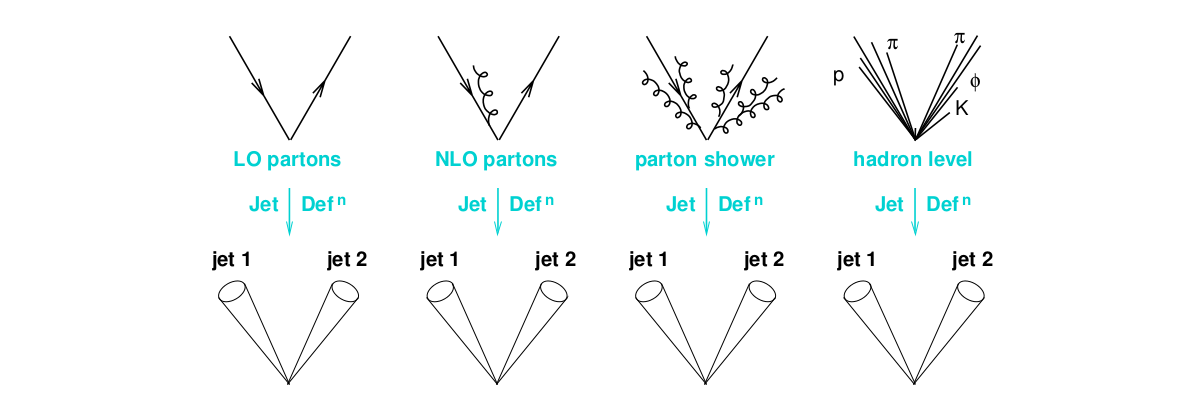
\includegraphics[width=1\textwidth]{Fig2/jetdefinition.png}
    \caption{The application of a jet definition to a variety of events that differ just through soft/collinear branching and hadronization should give identical jets in all cases~\cite{GavinLectures}.}
    \label{fig:jetdefinition}
  \end{center}
\end{figure}

Traditionally, jet algorithms have been classified into two categories: cone and sequential recombination algorithms. 

\subsubsection{Fixed cone jet finder in ATLAS}


 Cone-like algorithms are based on the collinear nature of gluon radiation and the parton shower described above. The decay products of quarks and gluons and their emissions will tend to form a cone of particles in the $\eta - \phi$ plane\footnote{In the ATLAS Coordinate System the azimuthal angle $\phi$ is measured around the beam axis, and the polar angle $\theta$ is the angle from the beam axis. The pseudorapidity is defined as $\eta = − \ln( \tan(\frac{\theta}{2}))$. The transverse momentum $\pt$ is defined in the plane transverse to the beam motion. The distance $\Delta R$ in the pseudorapidity-azimuthal angle space is defined as $\Delta R = \sqrt{ \Delta \eta^2  + \Delta \phi^2}$ . See section~\ref{sec:ATLASDetector}.} as they propagate outwards. 
The design of cone-like algorithms attempts to maximize the amount of energy present in a stable cone of fixed radius. 

In ATLAS the standard jet algorithm  for a long time was an iterative fixed-cone jet finder. 
First, it sorts all particles in the event according to their momentum, and identifies the one with largest $\pt$.  This is referred to as a seed particle.  Then a cone of radius $R_{cone}$ in  $\eta - \phi$ is drawn around the seed and all objects within a cone of $\Delta R < R_{cone}$ are combined with it. The direction of the sum of the momenta of those particles is identified and if it doesn't coincide with the seed direction then the sum is used as a new seed direction, and it iterates until the direction of the cone is stable (i.e, the direction of the sum of the cone contents coincides with the previous seed) and the resulting cone is called a jet . This type of algorithm is called  ``iterative'' since it iterates the cone direction. The jets found in this way can share part of their constituents. Jets with common constituents are merged if their shared $\pt$ is larger than 50\% of the $\pt$ of the softer jet.  Otherwise, the overlapping part is assigned to the harder jet (split).

A difficulty and major drawback in this procedure is the use of the transverse momentum of the particle to select the first seed. This definition is collinear unsafe, i.e. a splitting of the hardest particle into a nearly collinear pair can have the consequence that another, less hard particle, pointing in a different direction suddenly becomes the hardest in the event, leading to a different final set of jets\footnote{From the theoretical point of view, the splitting and merging procedures make this algorithm partially infrared safe, but the algorithm remains well defined only up to leading order of perturbation theory.}. There are many other variants of cone algorithms, and nearly all suffer from problems of either collinear safety, or infrared safety (an extra soft particle creates a new seed, which can lead to an extra stable cone being found). A fix for these problems came in a algorithm called Seedless Infrared Safe Cone (SISCone)~\cite{SISCone}.


\subsubsection{Sequential recombination algorithms}

Recombination algorithms are both collinear and infrared safe. For this reason, they can be used in calculations to any order in perturbation theory. %The term recombination is appropiate given that these algorithms work as if they were inverting the sequence of splittings of the parton shower. 
The term recombination is used since they attempt to follow the parton shower branchings which become progressively softer as the shower evolves. The resulting jet can be thought of as the final stage of this process and the algorithm is the device used to retrace the tree of sequential branchings.
In general, recombination algorithms operate by successively combining pairs of particles using a distance metric, $d_{ij}$.  At hadron colliders, due to the fact that one of the incoming partons may continue along the beam, for every pair of particles this metric is compared to a so-called ``beam distance'', $d_{iB}$, and only when  $d_{ij}<d_{iB}$ the particle pair is combined and considered for subsequent clustering steps. 

%ATLAS (and also CMS) has chosen the anti-$k_t$~\cite{antiktalg} algorithm as the default jet algorithm for use in physics analyses.  This recombination algorithm  %as well as the Cambridge-Achen (C$/$A) algorithm\footnote{C/A algorithm relies on angular ordering of emissions in order to reconstruct the shower by omitting the transverse momentum scales from $d_{ij}$ altogether.}~\cite{CamAchem} are extensions 
%is an extension of the original $k_t$ algorithm developed for the analysis of multi-jet events at $e^+ e^-$ colliders~\cite{JADE} and subsequently extended for use at hadron colliders~\cite{kt2,kt1}. In this thesis, the $k_t$ algorithm was used for jet substructure studies, see section~\ref{sec:substructure}.

\vspace{0.5cm}
\textbf{The $k_t$ algorithm}. The most common sequential recombination algorithm is the inclusive $k_t$ algorithm.  If was first implemented in the analysis of multi-jet events at $e^+ e^-$ colliders~\cite{JADE} and subsequently extended for use at hadron colliders~\cite{kt2,kt1}. 
It is instructive to compare both the original algorithm as well as the ultimate definition of the modern $k_t$ algorithm in order to identify relevant features of this algorithm.
The distance measure in the original  version is defined as: % \ref{eqn:origkt}
\begin{equation} 
d_{ij} = \frac{2E_i E_j (1- \cos \theta_{ij}) }{Q^2},
\label{eqn:origkt}
\end{equation}
where $Q$ is the total energy in the event, $E_i$ is the energy of particle $i$ and $\theta_{ij}$ the angle between particles $i$ and $j$. In the collinear limit, $d_{ij}$ is related to the relative transverse momentum between particles $i$ and $j$ (hence the name $k_t$ algorithm), normalized to the total visible energy.
The particles are combined if the minimum $d_{ij}$, $d_{min}$, is below a certain threshold, $y_{cut}$.  The jet multiplicity depends on the value of $y_{cut}$, as a lower value will result in more soft or collinear emissions surviving as jets. This is thus the first definition of an ``event shape'', this threshold marks the transition between two-jet events and three-jet events.

For a jet algorithm at a hadron collider, the notion of a beam distance is added. %the definition of $d_{ij}$ must account for the fact that partons scatter in a rest frame other than that of the center-of-mass of the colliding protons, unlike at an $e^+ e^-$ collider.  In particular, the notion of the beam distance is added in order to render the algorithm frame-independent. 
A distance scale, $\Delta R = \sqrt{\Delta y^2 +\Delta \phi^2}$, is introduced to define the typical radius for a jet, effectively replacing $y_{cut}$. In this case the particle distance metric becomes, % (\ref{eqn:kt})
%
\begin{equation} 
d_{ij} = \min(p^2_{ti},p^2_{tj}) \frac{\Delta R^2_{ij}}{R^2}
\label{eqn:kt}
\end{equation}
%
and the beam distance, 
%
\begin{equation}
d_{iB}=p^2_{ti}. 
\end{equation}
%
such that when no particle $j$ is found such that $\Delta R_{ij} < R$ then $i$ is promoted to the status of a jet.  

The formulation of the modern inclusive $k_t$ algorithm is formulated as follows:

\begin{enumerate}\addtolength{\itemsep}{-0.4\baselineskip}
\item  
Utilize the particle distance metric $d_{ij}$ defined in Eq.~\ref{eqn:kt}.
\item
Compute the minimum $d_{ij}$, $d_{min} = \min(d_{ij})$, among all particles.
\item
If  $d_{min} < d_{iB},d_{jB}$, then combine particles $i$ and $j$ and repeat from step 1.
\item
If $d_{ij} > d_{iB}$, then identify $i$ as a jet and remove it from the list.
\item
Continue until all particles are considered jets or have been clustered with other particles.
\end{enumerate}

 Jets built with this algorithm have quite irregular shapes, and particles with $\Delta R_{ij} > R$ can still be clustered within the jet. This is a problem when, for example, an irregularly shaped jet happens to extend into poorly instrumented detector regions. 

As defined, the $k_t$ algorithm clusters first objects that are either very close in angle or have very low transverse momentum. The fact that soft particles are clustered first is a another drawback of this definition since it  has the potential to introduce complications when the detector noise of energy density fluctuations are large.

A feature of the $k_t$ algorithm that is attractive is that it does not only produce jets but it also assigns a clustering sequence to the particles within the jet. It is possible then to undo the clustering and to look %inside the structure of the jet. 
back at the shower development history.  This has been exploited in a range of QCD studies, and also in searches of hadronic decays of boosted massive particles  and it will be used here for the search of two-pronged jets in gluon splitting.

The $k_t$ algorithm can be generalized by introducing the following particle-particle and particle-beam distance measures:
%
\begin{equation} 
d_{ij} = \min(p^{2n}_{ti},p^{2n}_{tj}) \frac{\Delta R^2_{ij}}{R^2}
 \label{eqn:generickt}
\end{equation}
%
\begin{equation}
d_{iB}=p^{2p}_{ti}. 
 \label{eqn:generickt2}
\end{equation}
%
where $p$ is a parameter which is 1 for the $k_t$ algorithm. Two different algorithms can be obtained from this: The Cambridge-Aachen (C$/$A) algorithm~\cite{CamAchem}, with $p=0$, and the anti-$k_t$ algorithm~\cite{antiktalg}, with $p=-1$. 

\textbf{The Cambridge-Aachen algorithm}. The C$/$A algorithm is obtained by choosing a value $p=0$ in Equations~\ref{eqn:generickt} and~\ref{eqn:generickt2}. This algorithm recombines objects close in $\Delta R$ iteratively and reflects the angular ordering of the QCD radiation.  It is ideally suited to reconstruct and decompose the various decay components of heavy objects like Higgs bossons or top quarks using subjet structure.


\textbf{The anti-$k_t$ algorithm}. Contrary to the $k_t$ algorithm, the anti-$k_t$ algorithm, so named because of the inverted power law in the particle and beam distance metrics in Equations~\ref{eqn:generickt} and~\ref{eqn:generickt2}, first clusters hard objects together %  This has several benefits in the context of high-luminosity hadron collisions.
which results in more regular jets with respect to the $k_t$ and C$/$A algorithms. This characteristic is illustrated for the $k_t$ and anti-$k_t$ algorithms in Fig.~\ref{fig:CatchmentAreaFig}.

\begin{figure}[tp]
\centering
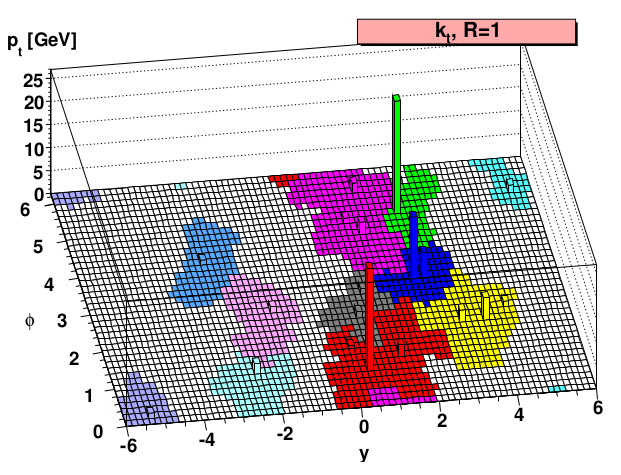
\includegraphics[width=0.49\textwidth]{areas_kt.png}
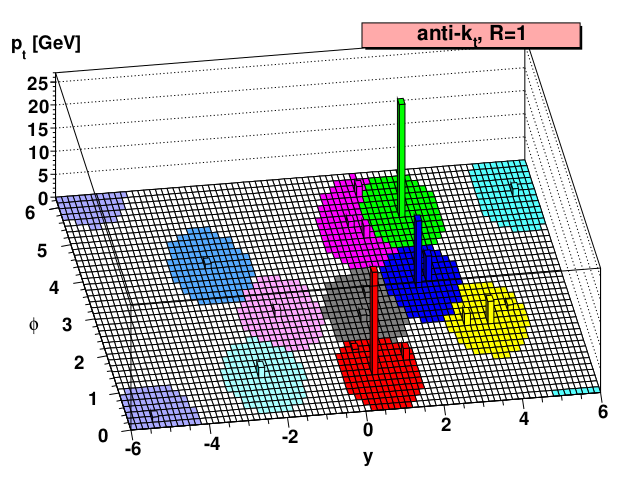
\includegraphics[width=0.49\textwidth]{areas-antikt.png}
\caption{A sample parton-level event, generated with {\sc Herwig}, clustered with the $k_t$ and anti-$k_t$ algorithms, illustrating the active area of the resulting jets~\cite{CatchmentArea}.}
\label{fig:CatchmentAreaFig}
\end{figure}


For this reason and the fact that this algorithm is less sensitive to soft emissions (see Chapter~\ref{ch:reco}) the anti-$k_t$ algorithm was chosen as the default jet algorithm for ATLAS analyses.

Note that the anti-$k_t$ algorithm does not provide useful information on jet substructure if a jet contains two hard cores, then the $k_t$ (or C/A) algorithms first reconstruct those hard cores and merge the resulting two subjets. The anti-$k_t$ will often first cluster the harder of the two cores and then gradually aglomerate the contents of the second hard core.

These algorithms, and more, are implemented in {\sc Fastjet}~\cite{fastjet} software package for jet-finding. 


%------------------------------------------------------------------------
\subsection{Jet substructure}\label{sec:substructure}
%------------------------------------------------------------------------

%The study of a quantity related to the distributions and multiplicity of particles in the event phase space led to the first evidence of jet structure, as pointed out in ref.~\cite{PhysRevLett.35.1609}. 
The first evidence of jet structure resulted from the study of the spacial distribution and multiplicity of particles in the event phase space in hadron production in $e^+ e^-$ collisions~\cite{PhysRevLett.35.1609}.
Generally, all final hadronic states in $pp/p\bar{p}/e^+e^-$ collisions can be explored in terms of the structure and shape of the event energy flow by means of the so called ``event shape'' variables. This family of variables attempts to extract information about the global geometry of an event, usually distinguishing between di-jet events and multijet final states. Such variables have been successfully utilized in many SM measurements and BSM searches, see for example~\cite{Abbiendi:2007aa,Aad:2012np}. 

Although very useful, event shape variables are not sensitive to the detailed structure and distribution of energy inside a particular jet. In SM and new physics searches, tools for the identification of individual objects that might be signature of new particles are desired. 
At the LHC, many of the particles considered to be heavy at previous accelerators will be frequently produced with a transverse momentum greatly exceeding their rest mass, like the electro-weak gauge bosons $W^\pm$ and $Z$, the top quark, the Higgs boson (or bosons) and possibly other new particles in the same mass range. These boosted objects, produced either by recoil against other energetic objects or from decays of even heavier BSM particles, upon decay can give rise to a highly collimated topology too close to be resolved by standard jet algorithms. 
%For example, when an unstable massive particle with large $\pt$ decays hadronically, the final state may be composed of a number of nearly collinear jets. These jets may be merged by a jet finder; %The decay products of boosted heavy quarks or bosons might be reconstructed as a single jet, 
A method for selecting these jets would allow for the study of their properties.   This interest led to the development of a wide range of %jet substructure techniques in the recent years. 
%For theses cases, 
sophisticated tools in the last years~\cite{boost2010,boost2010b} that allow the analysis of the substructure of the ensuing jet and reveal its heavy-particle origin.

  Jet substructure methods probe the internal structure of jets from a detailed study of its constituents. These techniques have been first implemented for distinguishing boosted SM hadronic objects from the background of jets initiated by light quarks and gluons, see for example~\cite{ATLASBoostedHbb},
%http://cdsweb.cern.ch/record/1201444/
but they have been also succesfully used in other applications, including separating quark jets from gluon jets~\cite{PhysRevLett.107.172001} and identifying boosted decay producs in new physics searches~\cite{PhysRevD.82.095012}.

%Jet shapes and jet algorithms in SCET, by Ellis, Vermillon, et all
Jet shapes, which are event shape-like observables applied to single jets, are an effective tool to measure the structure of individual jets~\cite{springerlink:10.1007/JHEP11(2010)101}.% {\bm ELEGIR REFERENCIA}. 
 The shape of a jet not only depends on the type of parton (quark or gluon) but is also sensitive to non-perturbative fragmentation effects and underlying event contributions~\cite{ATLASJetShapes}.


%from Jet substructure at the Tevatron and LHC
%Observables desinged to be sensitive to the internal structure of jets are expected to also be sensitive to pile-up. Large-radius jets, such as those used in the measurements of jet substructure, are naturally more susceptile to pile-up due to their larger catchment area~\cite{CatchmentArea}; the invariant mass of these large jets is particularly affected. %http://arxiv.org/abs/1009.1143
%Techniques for correcting these effects or mitigating their impact $-$such as the splitting and filtering procedure pioneered in ATLAS$-$  are essential in producing precision measurements for several of the analyses presented by the Tevatron and LHC experiments.  A more thorough review of these issues at ATLAS can be found in~\cite{DavidMillerThesis}


In chapter~\ref{ch:kinematic}, several distinguishing characteristics between jets originating from single $b$-quarks and jets containing two close-by  $b$-hadrons are determined using the techniques of jet substructure. 







%------------------------------------------------------------------------
\section{Heavy flavor jet production}%\label{sec:substructure}
%------------------------------------------------------------------------

%https://cdsweb.cern.ch/record/1425916/
Heavy flavor quarks enter in many collider searches, notably because they are produced in the decays of various SM particles (top quarks, the $Z$ boson and the Higgs boson, if light), and of numerous particles appearing in proposed extensions of the SM.
 In hadronic collisions, heavy flavour quark production may be subdivided into three classes depending on the number of heavy quarks participating in the hard scattering. The hard scatter is defined as the $2 \rightarrow 2$ subprocess with the largest virtuality (or shortest distance) in the hadron-hadron interaction~\cite{Norrbin:2000zc}.
%Ariel Thesis
%The $b$-quarks in $pp$ collisions are produced predominatly in pairs, as the result of the strong interaction between one parton from the proton and another parton from the antiproton.  The cross section for producing a $b$-quark in a $pp$ collision is calculated convoluting the perturbative parton cross section with the proton distribution functions:
%equation 1.3 Ariel's thesis
%blabla
%The contribution to the total $b\bar{b}$ cross section from higher order production mechanisms is comparable to that of the direct production.  This can be qualitatively understood because, for instance, the $gg\rightarrowgg$ cross section is about a factor of 100 larger than $gg\rightarrowb\bar{b}$, and the rate of gluon splitting to bottom quarks is proportional to $\alpha_s$, which is of the order of 0.1.



\begin{itemize}\addtolength{\itemsep}{-0.4\baselineskip}
\item
Heavy flavor creation (FCR): two heavy quarks are produced in the hard subprocess. Being $Q$ the heavy flavor quark, at leading order this process is described by $gg \rightarrow Q\bar{Q}$ and  $q\bar{q} \rightarrow Q\bar{Q}$.
\item
Heavy flavor excitation (FEX): the heavy flavour quark excitation can be depicted as an initial state gluon splitting into a heavy quark pair, where one of the heavy quarks subsequently enters the hard subprocess.
\item
Gluon splitting (GSP): no heavy quarks participate in the hard subprocess in this case, but they are produced in $g \rightarrow Q\bar{Q}$ branchings in the parton shower.
\end{itemize}

Example of Feynman diagrams for QCD $b$-quark production up to NLO are shown in Fig.~\ref{fig:qcd_diagrams}.

%
\begin{figure}[h!]
\centering
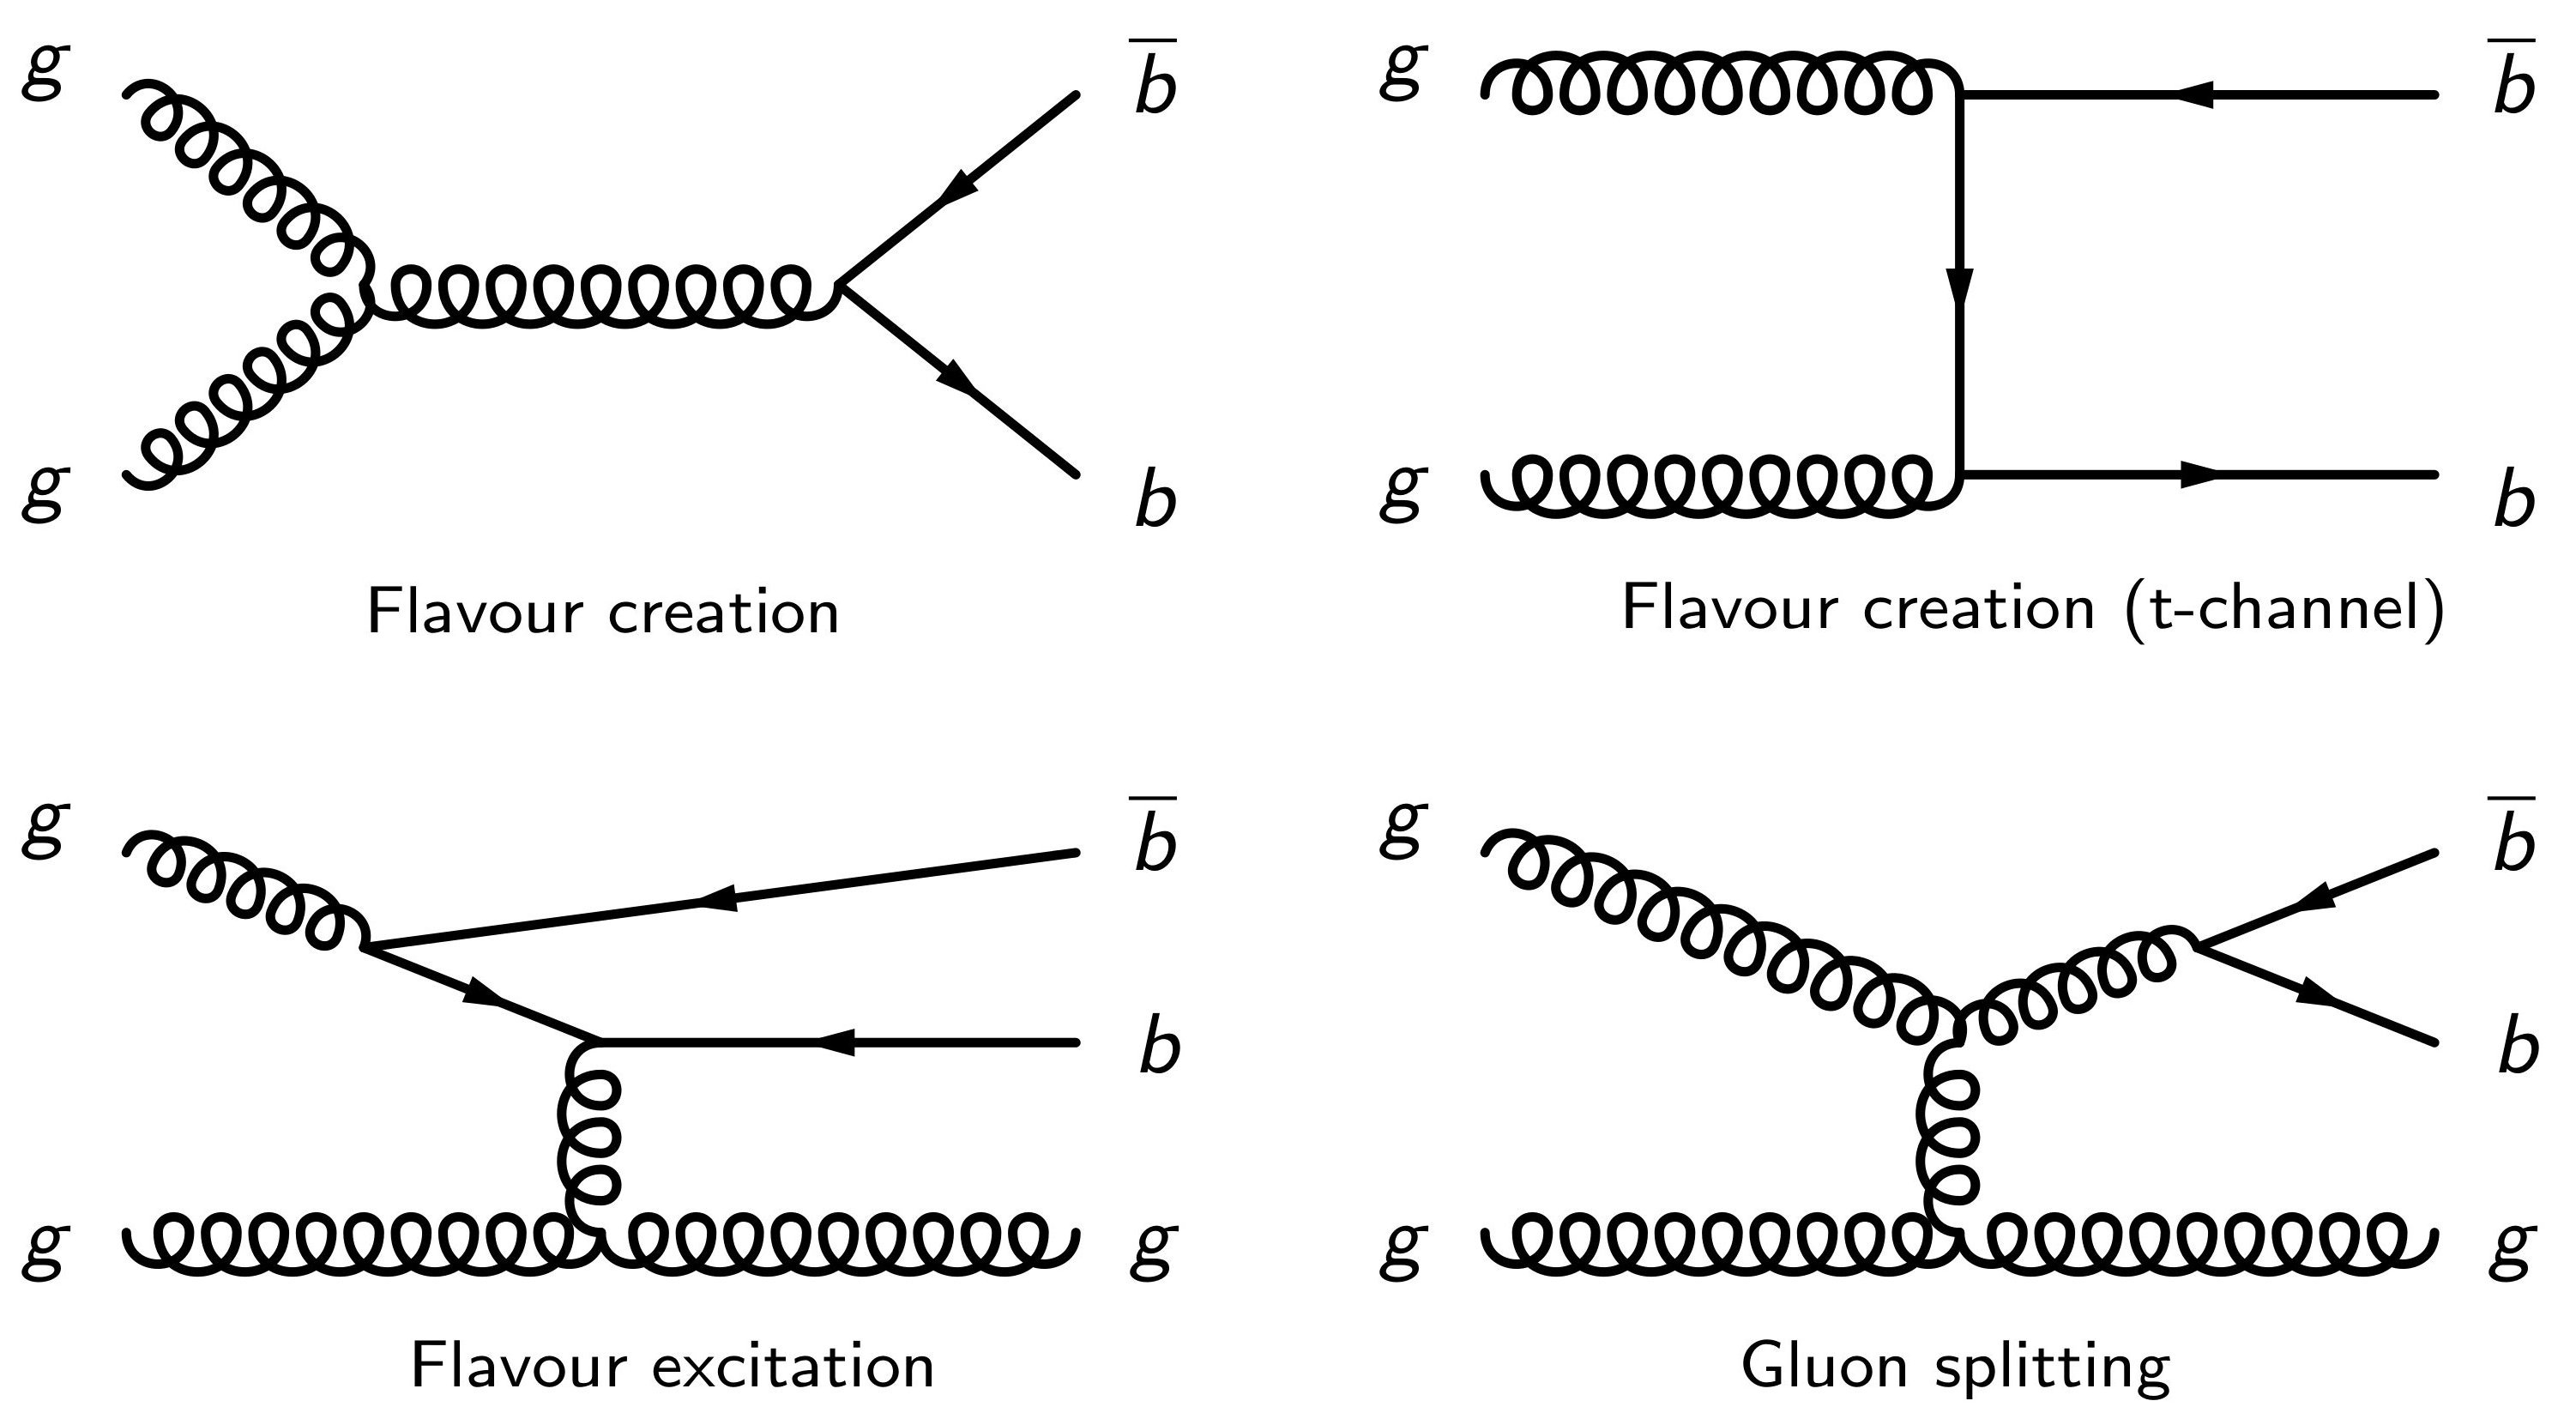
\includegraphics[width=0.32\textwidth,viewport=0 880 1500 1600,clip]{FIGS/bb_diagrams.jpg}
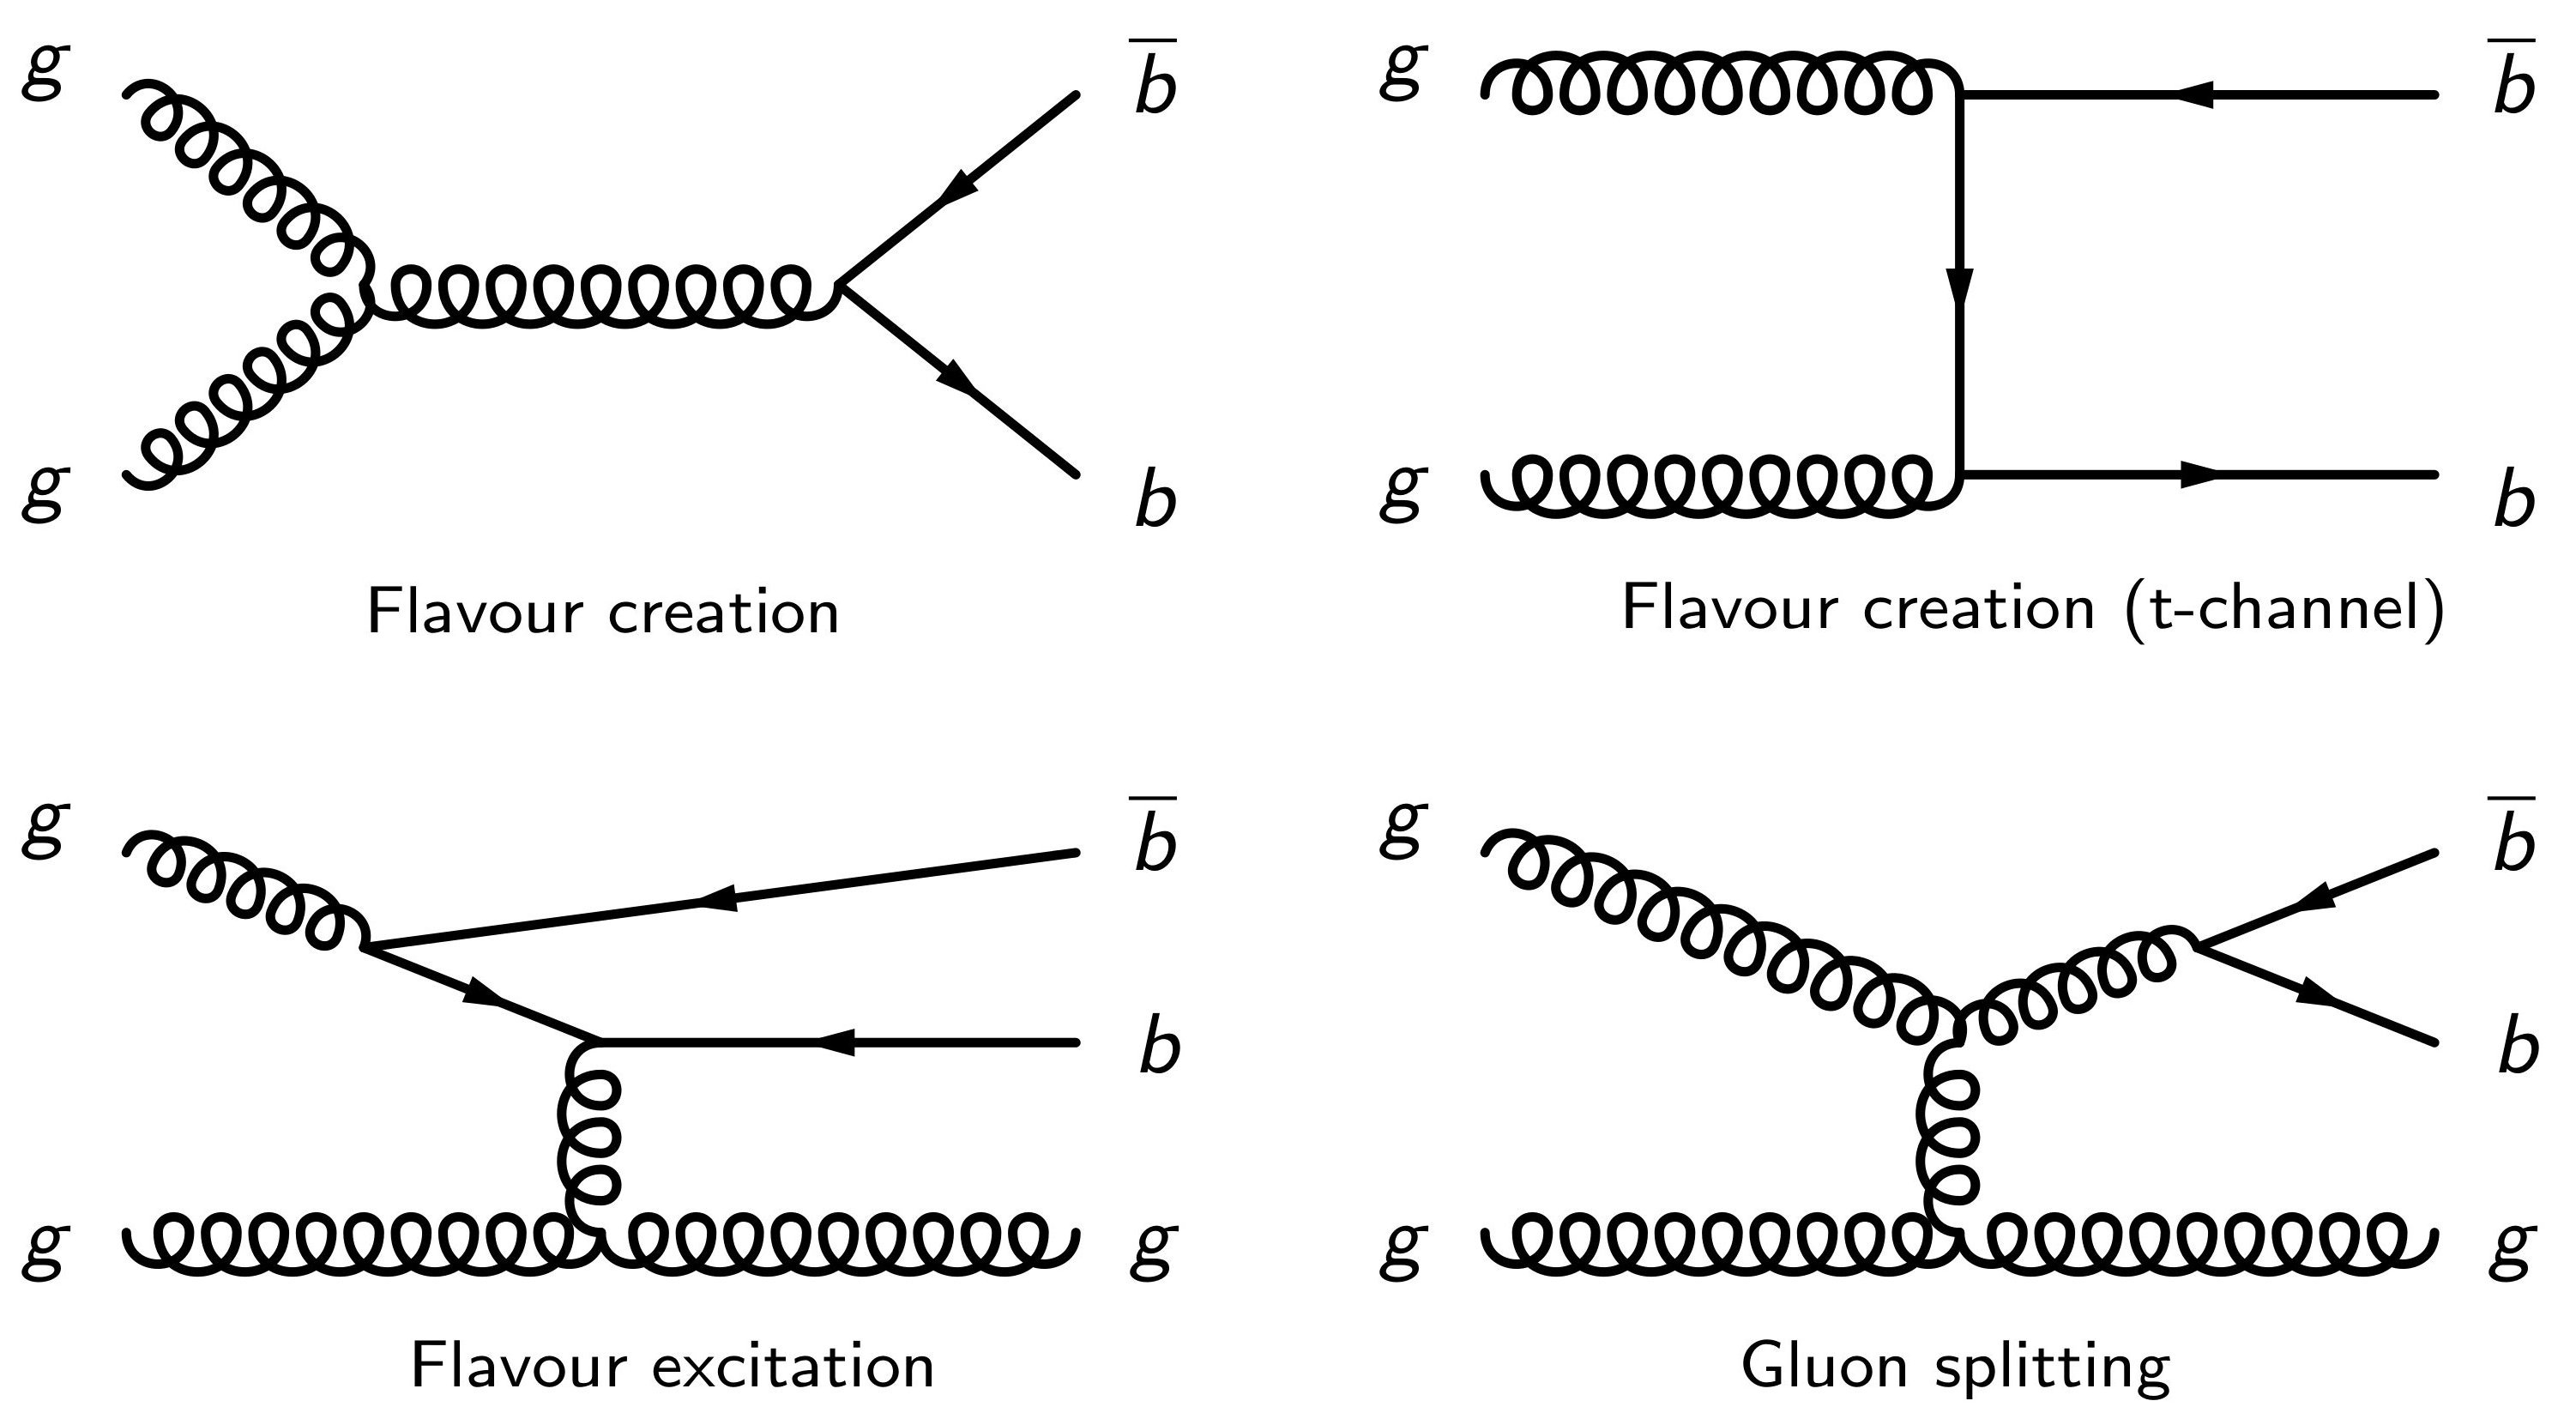
\includegraphics[width=0.32\textwidth,viewport=1600 0 3100 820,clip]{FIGS/bb_diagrams.jpg}
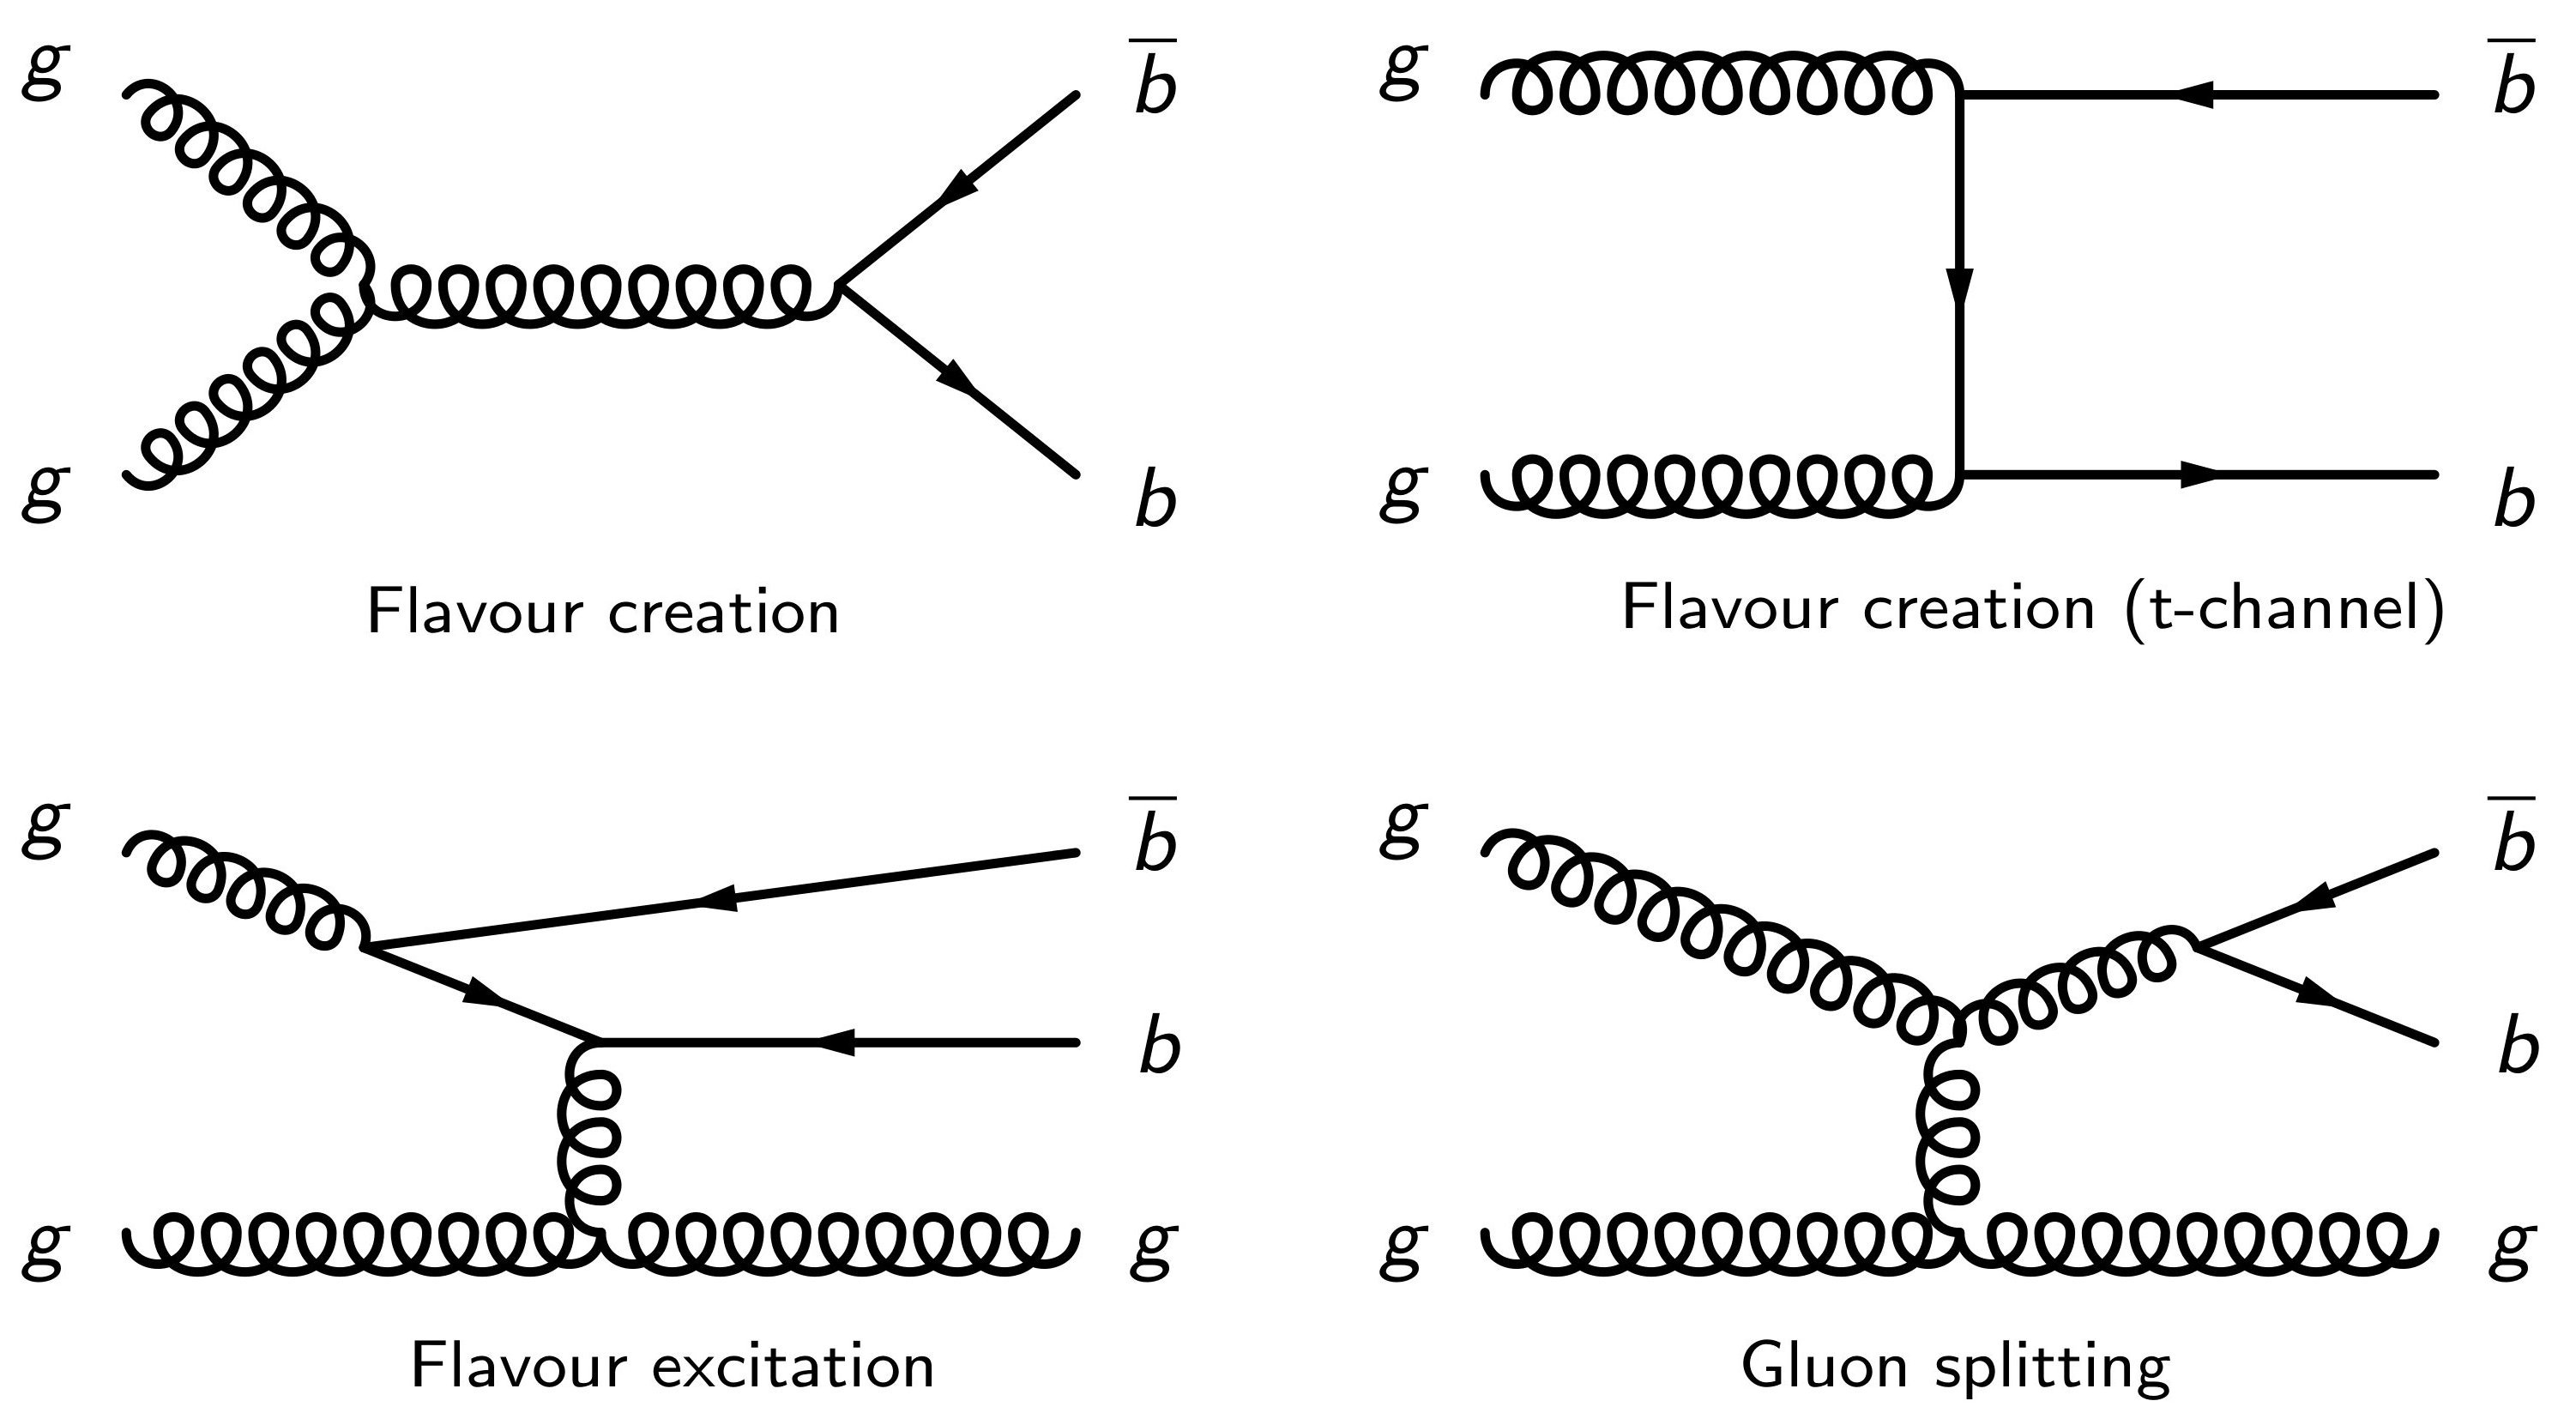
\includegraphics[width=0.32\textwidth,viewport=0 0 1500 820,clip]{FIGS/bb_diagrams.jpg}
\caption{Representative diagrams of the three channels contributing to QCD $b$-quark production up to NLO. The flavour creation channel (left) is the only one present at LO. At NLO, two new channels open up, referred to as gluon splitting (center) and  flavour excitation (right).}
\label{fig:qcd_diagrams}
\end{figure}
%

The definition above is not strict, but can be used as a basis for the understanding of the characteristics of heavy flavour quark production.

%From  Ariel's thesis
Final state $b$-quarks hadronize into $b$-hadrons. During the fragmentation process, other particles will also be produced along with the $b$-hadron, giving rise to $b$-jets. Directly produced $b$-jets are $\pt$ balanced and back-to-back in the azimuthal angle $\phi$. However they are not 3-D balanced because $b$-jets may be boosted in the $z$ direction due to the different proton momentum fractions carried by the initial partons.  In the flavor excitation process, the $b$-quark which does not participate in the hard scatter belongs to the underlying event, resulting in a forward (large $\eta$) $b$-jet.  The angular $\Delta \phi$ separation between the two $b$-jets is therefore expected to be flat.  Gluon splitted $b$-jets are expected to be collinear since they originate from the splitting of a gluon and will tend to be identified as a same hadronic jet. The azimuthal separation between the two gluon splitted $b$-jets thus peaks at small angles.



%%%%%%%%%%%%%%%%%%%%%%%%%%%%%%%%%%%%%%%%%%%%%%%%%%%%%%%%%%%%%%%%%%%%%%
%{\em The measurement of the inclusive $b$-jet spectrum}
%%%%%%%%%%%%%%%%%%%%%%%%%%%%%%%%%%%%%%%%%%%%%%%%%%%%%%%%%%%%%%%%%%%%%%

The simplest and most fundamental measurement of heavy-quark jet production is
the inclusive heavy-quark jet spectrum, which is dominated by pure QCD contributions. 
Studies of QCD bottom production are important in their own right because of the correspondence between parton level production and the observed hadron level, and their potential to provide information on the $b$-quark parton distribution function, a component of the proton structure thought to be generated entirely perturbatively from the QCD evolution equations of the other flavours. The theoretical calculation of the inclusive $b$-jet spectrum presents rather important uncertainties ($\sim 50\%$), considerably larger than those for the light jet inclusive spectrum ($\sim 10-20\%$)~\cite{Frixione:1996nh}. 

%Paper by Salam, Banfi and Zanderighi
%The measurement suggestion that motivated our development: a b-jet xsection that excludes double-B jets: 
%a. Full NLO calculation of the inclusive b-jet spectrum yields a K-factor=6-10.
%b. Herwig analysis shows that FEX and GSP contributions are much larger than FCR. This is due to strong enhancement from collinear logarithms.
%Proposal: move to inclusive flavour-kt b-jet xsection where bb-jets are not counted. Theoretical uncertainties are substantially reduced
%a. Flavour-kt b-jet xsection is free of final-state (GSP) logarithms
%b. Initial-state (FEX) collinear logarithms can be resummed if one uses a b-quark PDF
A review of the origin of these uncertainties is presented by Banfi, Salam and Zanderighi in reference~\cite{Salam.AccurateHQ}.  They arise from the poor convergence of the perturbative series, as evidenced by a large value of the $K$-factor, the ratio of the next-to-leading order (NLO) to the leading order (LO) cross section, in the $\pt$ range covered by the LHC.  This is illustrated in Fig.~\ref{fig:bjets_qcd}.  The observed $K$ values (6 to 10) indicate that the NLO result cannot be an accurate approximation to the full result. It is for this reason that the scale dependence (middle panel in Fig.~\ref{fig:bjets_qcd}) is large. 

\begin{figure}[tp]
\centering
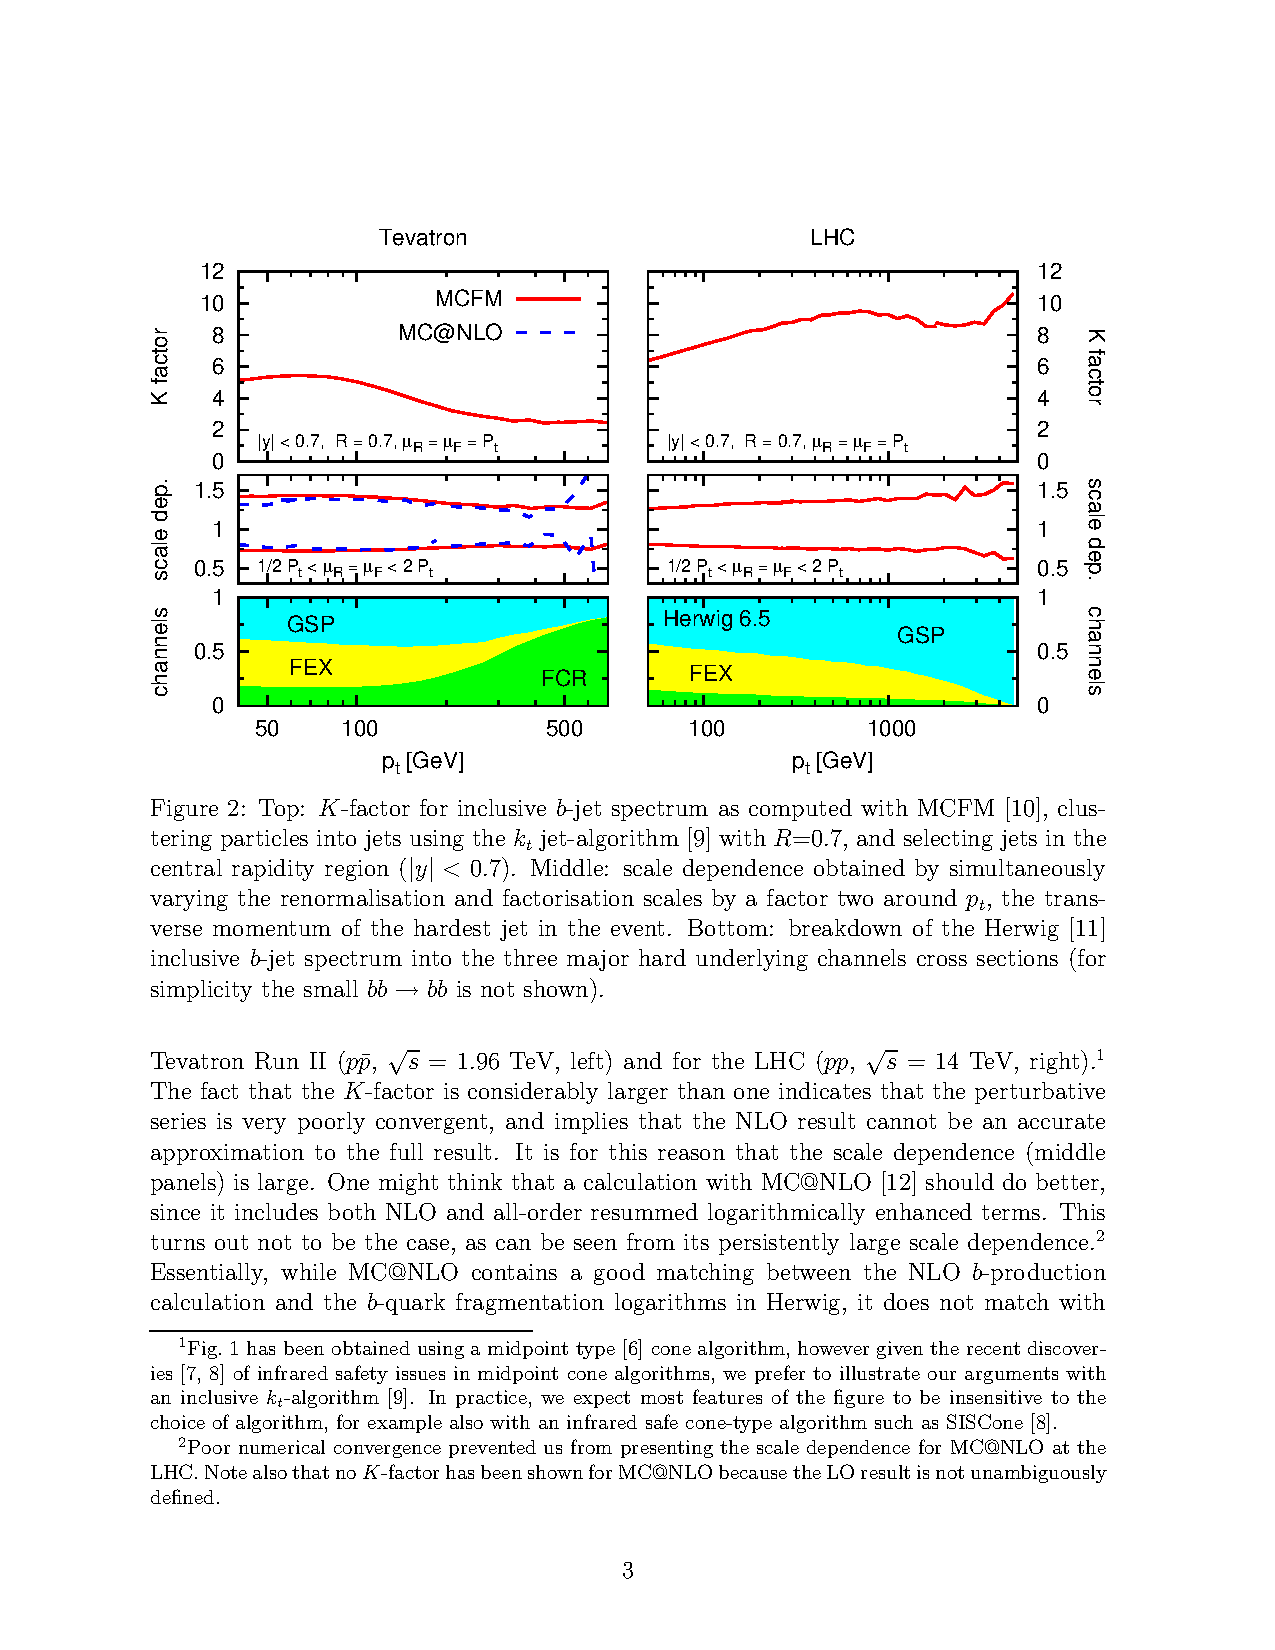
\includegraphics[height=0.7\textwidth,viewport=300 410 530 690,clip]{FIGS/bjets_qcd.pdf}
  \caption{Top: $K$-factor for inclusive $b$-jet spectrum taken from~\cite{Salam.AccurateHQ}, clustering particles into jets using the $k_t$   jet-algorithm~\cite{kt1}  with $R$=0.7, and selecting jets in the central rapidity region ($|y| <0.7$). Middle: scale dependence obtained by simultaneously varying the renormalisation and factorisation scales by a factor two around $\pt$, the transverse momentum of the hardest jet in the event. Bottom: breakdown of the Herwig \cite{Herwig} inclusive $b$-jet spectrum into the three major underlying channels, flavor creation (FCR) flavor excitation (FEX) and gluon splitting (GSP).}
  \label{fig:bjets_qcd}
\end{figure}

The fact that the perturbative series is very poorly convergent is related to the different channels for heavy quark production. 
While at LO only the FCR channel is present, at NLO the FEX and GSP channels open up\footnote{It is sometimes stated that it makes no sense, beyond LO, to separately discuss the different channels, for example because diagrams for separate channels interfere. However, each channel is associated with a different structure of logarithmic enhancements, $\ln^n (\pt / m_b )$, and so there is distinct physical meaning associated with each channel.}.  %often referred to as ``flavour excitation'' (FEX) and ``gluon splitting'' (GSP), 
 In the gluon splitting process, one of the final-state light partons (at NLO always a gluon) splits collinearly into a $b\bar{b}$ pair that a clustering algorithm can classify within the same jet. A jet containing both $b$ and $\bar{b}$ is considered to be just a $b$-jet in standard definitions.

The various channels can be approximately separated in a parton shower Monte Carlo generator such as {\sc Herwig} or {\sc Pythia}. These MC generators include NLO effects, and 
%these,  where 
one can determine the underlying hard process from the event record.  Their relative contributions to the total $b$-jet spectrum are shown in the bottom panel of Fig.~\ref{fig:bjets_qcd}. It is found that the LO channel has a much smaller contribution than the FEX and the GSP channels, which
receive strong enhancement from collinear logarithms, %~\cite{GSP} 
going as $\alpha_s^2 (\alpha_s \ln( \pt / m_b))^n$ for flavour excitation~\cite{Altarelli1977298} 
and $\alpha_s^2 \cdot \alpha_s^n \ln^{2n-1}(\pt/m_b)$ for gluon splitting ($n\ge 1$)~\cite{Seymour1995163}.
%Also http://arxiv.org/abs/hep-ph/0308284 and http://arxiv.org/abs/hep-ph/0404242

Ref.~\cite{Salam.AccurateHQ} proposes a new observable to free the heavy-flavour spectrum calculation from collinear logarithms, and improve the accuracy of the theoretical prediction,
%for improving the accuracy of the prediction of the heavy-flavour spectrum 
by not including in the production cross-section the contribution from double $b$ jets. Final-state logarithms are removed by employing a recently developed jet reconstruction scheme, the flavour-$k_t$ algorithm~\cite{flavorkt}, which maintains the correspondence between partonic flavour and jet flavour. Specifically, jets containing a $b$-quark and a $b$-antiquark, which in a parton shower MC generator are produced $\sim95\%$ of the time by the GSP channel, are labeled in an IR-safe way as light jets and removed from the $b$-jet spectrum.
The initial-state (FEX) collinear logarithms can be resummed by using a $b$-quark parton distribution functions.
With this algorithm the $K$-factor for the differential heavy-jet spectrum cross-section is shown not to exceed a value of $K=1.4$, with a factor of four reduction in the theoretical (scale variation) uncertainties.



%%%%%%%%%%%%%%%%%%%%%%%%%%%%%%%%%%%%%%%%%%%%%%%%%%%%%%%%%%%%%%%%%%%%%%%
%{\em Rejection of background in Standard Model analyses and beyond-SM searches}
%%%%%%%%%%%%%%%%%%%%%%%%%%%%%%%%%%%%%%%%%%%%%%%%%%%%%%%%%%%%%%%%%%%%%%%

Succesfully identifying jets with two $b$-hadrons, the products of the $b$-quark or $b$-antiquark hadronization, 
%Efficient tagging of merged $b$-jets 
can also provide an important handle to understand, estimate and/or reject $b$-tagged backgrounds to SM and new physics searches at the LHC.

%Within the Standard Model (SM) a range of QCD production channels exists for heavy-quark jets, either via pure QCD production or in association with heavy bosons ($W, Z, H$). These channels are expected to produce a mixture of single-$B$ and double $b$-hadron jets. On the other hand, 
%These are expected to produce essentially single-$B$ jets. The ability to distinguish double- from single-$B$ jets is thus of wide application. 
SM physics analyses that rely on the presence of single $b$-jets in the final state, such as top quark physics, either in the $t\bar{t}$ or the single top channels, and associated Higgs production: $WH\rightarrow\ell\nu b\bar{b}$ and $ZH\rightarrow\nu\nu b\bar{b}$,  suffer from  %backgrounds that can be in part removed by a merged $b$-jet tagger. 
the reducible background from QCD, which can produce double $b$-hadron jets as discussed above, and the irreducible background due to $W$ bosons produced in association with $b$-quarks.
Figure~\ref{fig:Wplusb} shows the two diagramas %leading order processes 
for $W+b$ production. %that give rise to $W$ bosons with at least one $b$-jet. 

\begin{figure}[htbp]
  \begin{center}
      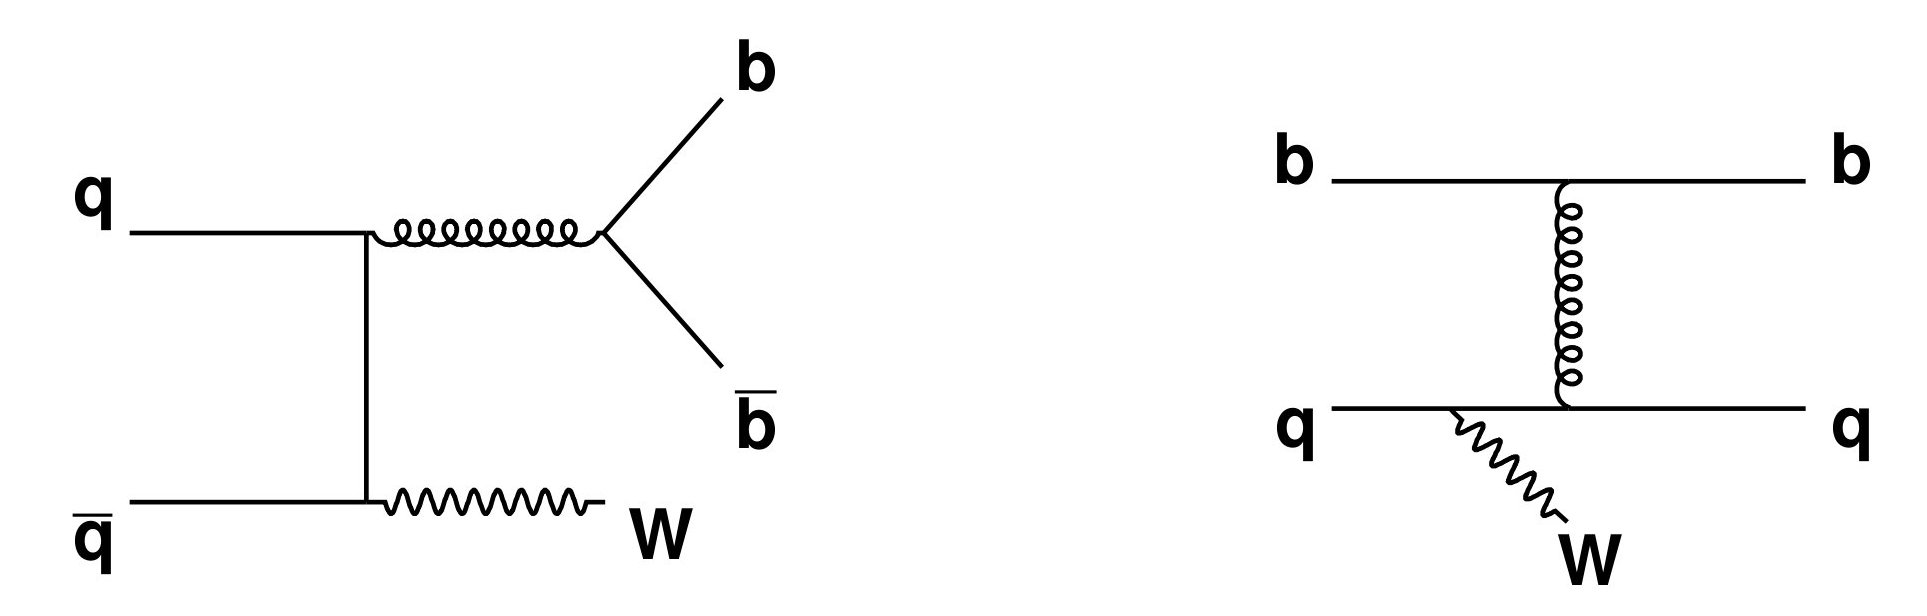
\includegraphics[width=0.6\textwidth]{FIGS/Wbb_diagram.jpg}
    \caption{Feynman diagrams for $W$ production in association with $b$ quarks.}
    \label{fig:Wplusb}
  \end{center}
\end{figure}

While at LO only single $b$-jets are present, at NLO jets containing two $b$-hadrons are expected due to the contribution of a diagram containing a $gb\bar{b}$ vertex. The $b$-quark pair is produced at small angles and can be often reconstructed as one merged jet.
%In the first process, which can be thought of as a higher order correction to $W$ + jets production, the $b$ quark pair is produced at small angles by gluonsplitting and can often be reconstructed as a merged jet.




The relevance of double $b$-hadron jets is supported by NLO calculations of the production of $W$ bosons and two jets with at least one $b$ quark at the LHC for jet $\pt > 25$ GeV, and $|\eta| < 2.5$~\cite{Campbell:2006} indicate that the cross section for $W(b\bar{b})j$ is almost a factor of two higher than $Wb\bar{b}$, and about a third of $Wbj$, where  $W(b\bar{b})j$ denotes the case in which the two $b$ quarks are merged into the same jet. 

Jets containing a single $b$-quark or antiquark %Single $b$-jets 
also enter in many BSM collider searches, notably because $b$-quarks are produced in the decays both of heavy SM particles (top quarks, the $Z$ boson and the Higgs boson), and of particles appearing in proposed extensions of the SM.  %The ability to distinguish single $b$-jets from jets containing two $b$-hadrons is thus here of wide application to reduce SM backgrounds giving rise to close-by $b\bar{b}$ pairs.
%New physics searches with $b$-quarks in the final state also benefit from rejection of QCD and $W+b$ backgrounds which have $b$-jets arising from gluon splitting. 
 An example is the search for supersymmetry in the framework of generic $R$-parity conserving models~\cite{ATLAS-CONF-2011-098}. The superpartners of quarks and gluons could be copiously produced via the strong interaction at the LHC. The partners of the right- and left-handed quarks, \~{q}$_{L}$ and  \~{q}$_{R}$, can mix to form two mass eigenstates and, since mixing is proportional to the corresponding fermion masses, it becomes more important for the third generation producing sbottom and stop significantly lighter than the other squarks. In this model, thus, sbottom and stop production is expected to dominate. As they chain decay to $b$-quarks and the lightest supersymmetric particle, the signature for this channel is missing transverse energy %\met\ 
plus (single) $b$-jets. The ability to distinguish single $b$-jets from jets containing two $b$-hadrons is thus here of wide application to reduce SM backgrounds giving rise to close-by $b\bar{b}$ pairs. %merged $b$-jets.


%%%%%%%%%%%%%%%%%%%%%%%%%%%%%%%%%%%%%%%%%%%%%%%%%%%%%%%%%%%%%%%%%%%%%%%%
% {\em Study of jet substructure and boosted objects}
%%%%%%%%%%%%%%%%%%%%%%%%%%%%%%%%%%%%%%%%%%%%%%%%%%%%%%%%%%%%%%%%%%%%%%%

   The study of $b\bar{b}$ jets from gluon splitting is an ideal testbed for exploring jet substructure in data, as it provides a large supply of boosted, merged jets. Furthermore, understanding $g\rightarrow b \bar{b}$ jets is important as they are themselves the background to boosted object searches, like $Z\rightarrow b\bar{b}$ or $H\rightarrow b \bar{b}$.  %In particular, it has recently been suggested~\cite{Butterworth:2008iy} that $WH$ and $ZH$ production become potential discovery and analysis channels by restricting one’s attention to the $\sim5$\% of events in which the vector and Higgs bosons have large transverse momentum, ${\pt}_H\gtrsim200$ GeV. 
Understanding the much more common QCD events with double $b$-hadron jets will be essential before attempting to measure more rare final states.


%%%%%%%%%%%%%%%%%%%%%%%%%%%%%%%%%%%%%%%%%%%%%%%%%%%%%%%%%%%%%%%%%%%%%%%%%
%  Gluon splitting fraction in hadronic Z decays (SLD, DELPHI)
%\subsubsection{Gluon splitting Measurements}
%%%%%%%%%%%%%%%%%%%%%%%%%%%%%%%%%%%%%%%%%%%%%%%%%%%%%%%%%%%%%%%%%%%%%%%5%


%The average multiplicity of $b\bar{b}$ pairs from gluons in hadronic $Z^0$ decays was first measured by DELPHI experiment at LEP. The analysis was performed by looking for secondary vertex production in 4-jet events. The average rate was found to be (0.21$\pm$0.11(stat.)$\pm$0.09(syst.))\%~\cite{Abreu:1997nf}.

%The rate of gluon splitting into bottom quarks, $g \rightarrow b\bar{b}$, was also measured by the Stanford Linear Collider (SLC) Large Detector (SLD), in hadronic $Z^0$ decays collected from 1996 to 1998~\cite{Abe:1999vw}. Following a similar procedure, the rate per hadronic event was found to be (3.7$\pm$0.71(stat.)$\pm$0.66(syst.))$\times$10$^{-3}$. In order to improve singal/background ratio, topological information was used. % A cut on $cos\theta$ between the two most energetic jets, jets 1 and 2 is performed to remove $b\bar{b}$ background with one $b$-jet splitting into two giving rise to two very collinear vertex axis.  Secondly, the variable $|cos\alpha_{1234}|$, where $alpha_{1234}$ is the angle between the plane formed by jets 1 and 2 and the plane formed by jets 3 and 4, is used to supress the $b\bar{b}$ background. This variable is useful to separate $g\rightarrowb\bar{b}$ events because the radiated virtual gluon in the process $Z^0 \rightarrow q\bar{q}g $ is polarized in the plane of the three-parton event, and this is reflected in the subsequent splitting, by strongly favoring $g\rightarrowb\bar{b}$ emission out of this plane.

 %The probability for secondary production of a bottom quark pair from a gluon per hadronic $Z^0$ decay in $e^+e^-$ annihilation, 
%\begin{equation} 
%g_{b\bar{b}} = \frac{N(Z^0 \rightarrow q\bar{q}g, g \rightarrow b\bar{b} )}{N(Z^0 \rightarrow hadrons)}
%\end{equation} 
%is expected to be very small, since the gluon must have sufficient energy to produce the bottom quark pair. 



%%% ATLAS Flavor composition analyses 
%%% !!!!!!!

